% Template for PLoS
%DIF LATEXDIFF DIFFERENCE FILE
%DIF DEL attack-old.tex   Mon May 21 14:08:36 2018
%DIF ADD attack.tex       Wed May 23 15:29:52 2018
% Version 3.5 March 2018
%
% % % % % % % % % % % % % % % % % % % % % %
%
% -- IMPORTANT NOTE
%
% This template contains comments intended 
% to minimize problems and delays during our production 
% process. Please follow the template instructions
% whenever possible.
%
% % % % % % % % % % % % % % % % % % % % % % % 
%
% Once your paper is accepted for publication, 
% PLEASE REMOVE ALL TRACKED CHANGES in this file 
% and leave only the final text of your manuscript. 
% PLOS recommends the use of latexdiff to track changes during review, as this will help to maintain a clean tex file.
% Visit https://www.ctan.org/pkg/latexdiff?lang=en for info or contact us at latex@plos.org.
%
%
% There are no restrictions on package use within the LaTeX files except that 
% no packages listed in the template may be deleted.
%
% Please do not include colors or graphics in the text.
%
% The manuscript LaTeX source should be contained within a single file (do not use \input, \externaldocument, or similar commands).
%
% % % % % % % % % % % % % % % % % % % % % % %
%
% -- FIGURES AND TABLES
%
% Please include tables/figure captions directly after the paragraph where they are first cited in the text.
%
% DO NOT INCLUDE GRAPHICS IN YOUR MANUSCRIPT
% - Figures should be uploaded separately from your manuscript file. 
% - Figures generated using LaTeX should be extracted and removed from the PDF before submission. 
% - Figures containing multiple panels/subfigures must be combined into one image file before submission.
% For figure citations, please use "Fig" instead of "Figure".
% See http://journals.plos.org/plosone/s/figures for PLOS figure guidelines.
%
% Tables should be cell-based and may not contain:
% - spacing/line breaks within cells to alter layout or alignment
% - do not nest tabular environments (no tabular environments within tabular environments)
% - no graphics or colored text (cell background color/shading OK)
% See http://journals.plos.org/plosone/s/tables for table guidelines.
%
% For tables that exceed the width of the text column, use the adjustwidth environment as illustrated in the example table in text below.
%
% % % % % % % % % % % % % % % % % % % % % % % %
%
% -- EQUATIONS, MATH SYMBOLS, SUBSCRIPTS, AND SUPERSCRIPTS
%
% IMPORTANT
% Below are a few tips to help format your equations and other special characters according to our specifications. For more tips to help reduce the possibility of formatting errors during conversion, please see our LaTeX guidelines at http://journals.plos.org/plosone/s/latex
%
% For inline equations, please be sure to include all portions of an equation in the math environment.  For example, x$^2$ is incorrect; this should be formatted as $x^2$ (or $\mathrm{x}^2$ if the romanized font is desired).
%
% Do not include text that is not math in the math environment. For example, CO2 should be written as CO\textsubscript{2} instead of CO$_2$.
%
% Please add line breaks to long display equations when possible in order to fit size of the column. 
%
% For inline equations, please do not include punctuation (commas, etc) within the math environment unless this is part of the equation.
%
% When adding superscript or subscripts outside of brackets/braces, please group using {}.  For example, change "[U(D,E,\gamma)]^2" to "{[U(D,E,\gamma)]}^2". 
%
% Do not use \cal for caligraphic font.  Instead, use \mathcal{}
%
% % % % % % % % % % % % % % % % % % % % % % % % 
%
% Please contact latex@plos.org with any questions.
%
% % % % % % % % % % % % % % % % % % % % % % % %

\documentclass[10pt,letterpaper]{article}
\usepackage[top=0.85in,left=2.75in,footskip=0.75in]{geometry}

% amsmath and amssymb packages, useful for mathematical formulas and symbols
\usepackage{amsmath,amssymb}

% Use adjustwidth environment to exceed column width (see example table in text)
\usepackage{changepage}

% Use Unicode characters when possible
\usepackage[utf8x]{inputenc}

% textcomp package and marvosym package for additional characters
\usepackage{textcomp,marvosym}

% cite package, to clean up citations in the main text. Do not remove.
\usepackage{cite}

% Use nameref to cite supporting information files (see Supporting Information section for more info)
\usepackage{nameref,hyperref}

% line numbers
\usepackage[right]{lineno}

% ligatures disabled
\usepackage{microtype}
\DisableLigatures[f]{encoding = *, family = * }

% color can be used to apply background shading to table cells only
\usepackage[table]{xcolor}

% array package and thick rules for tables
\usepackage{array}

% create "+" rule type for thick vertical lines
\newcolumntype{+}{!{\vrule width 2pt}}

% create \thickcline for thick horizontal lines of variable length
\newlength\savedwidth
\newcommand\thickcline[1]{%
  \noalign{\global\savedwidth\arrayrulewidth\global\arrayrulewidth 2pt}%
  \cline{#1}%
  \noalign{\vskip\arrayrulewidth}%
  \noalign{\global\arrayrulewidth\savedwidth}%
}

% \thickhline command for thick horizontal lines that span the table
\newcommand\thickhline{\noalign{\global\savedwidth\arrayrulewidth\global\arrayrulewidth 2pt}%
\hline
\noalign{\global\arrayrulewidth\savedwidth}}


% Remove comment for double spacing
\usepackage{setspace} 
\doublespacing

% Text layout
\raggedright
\setlength{\parindent}{0.5cm}
\textwidth 5.25in 
\textheight 8.75in

% Bold the 'Figure #' in the caption and separate it from the title/caption with a period
% Captions will be left justified
\usepackage[aboveskip=1pt,labelfont=bf,labelsep=period,justification=raggedright,singlelinecheck=off]{caption}
\renewcommand{\figurename}{Fig}

% Use the PLoS provided BiBTeX style
\bibliographystyle{plos2015}

% Remove brackets from numbering in List of References
\makeatletter
\renewcommand{\@biblabel}[1]{\quad#1.}
\makeatother



% Header and Footer with logo
\usepackage{lastpage,fancyhdr,graphicx}
\usepackage{epstopdf}
%\pagestyle{myheadings}
\pagestyle{fancy}
\fancyhf{}
%\setlength{\headheight}{27.023pt}
%\lhead{\includegraphics[width=2.0in]{PLOS-submission.eps}}
\rfoot{\thepage/\pageref{LastPage}}
\renewcommand{\headrulewidth}{0pt}
\renewcommand{\footrule}{\hrule height 2pt \vspace{2mm}}
\fancyheadoffset[L]{2.25in}
\fancyfootoffset[L]{2.25in}
\lfoot{\today}

\usepackage{booktabs} % For formal tables
\usepackage{epigraph}
\usepackage{afterpage}
\usepackage{tikz}
\usepackage{soul}
\usepackage[framemethod=tikz]{mdframed}
\usetikzlibrary{arrows,chains,decorations.pathreplacing}
\usepackage{pifont} % http://ctan.org/pkg/pifont
\usepackage{amsthm}

%% Include all macros below

\newcommand{\beq}{\begin{eqnarray}}
\newcommand{\eeq}{\end{eqnarray}}
\newcommand{\bhlpar}{\begin{mdframed}[innerleftmargin=0,innerrightmargin=0,hidealllines=true,backgroundcolor=yellow!20]}
\newcommand{\ehlpar}{\end{mdframed}}
\DeclareMathOperator{\wbf}{wBF}
\newtheorem{theorem}{Theorem}
\newcommand{\cmark}{\ding{51}}
\newcommand{\xmark}{\ding{55}}

\newcommand{\lorem}{{\bf LOREM}}
\newcommand{\ipsum}{{\bf IPSUM}}


%% END MACROS SECTION


%DIF PREAMBLE EXTENSION ADDED BY LATEXDIFF
%DIF UNDERLINE PREAMBLE %DIF PREAMBLE
\RequirePackage[normalem]{ulem} %DIF PREAMBLE
\RequirePackage{color}\definecolor{RED}{rgb}{1,0,0}\definecolor{BLUE}{rgb}{0,0,1} %DIF PREAMBLE
\providecommand{\DIFaddtex}[1]{{\protect\color{blue}\uwave{#1}}} %DIF PREAMBLE
\providecommand{\DIFdeltex}[1]{{\protect\color{red}\sout{#1}}}                      %DIF PREAMBLE
%DIF SAFE PREAMBLE %DIF PREAMBLE
\providecommand{\DIFaddbegin}{} %DIF PREAMBLE
\providecommand{\DIFaddend}{} %DIF PREAMBLE
\providecommand{\DIFdelbegin}{} %DIF PREAMBLE
\providecommand{\DIFdelend}{} %DIF PREAMBLE
%DIF FLOATSAFE PREAMBLE %DIF PREAMBLE
\providecommand{\DIFaddFL}[1]{\DIFadd{#1}} %DIF PREAMBLE
\providecommand{\DIFdelFL}[1]{\DIFdel{#1}} %DIF PREAMBLE
\providecommand{\DIFaddbeginFL}{} %DIF PREAMBLE
\providecommand{\DIFaddendFL}{} %DIF PREAMBLE
\providecommand{\DIFdelbeginFL}{} %DIF PREAMBLE
\providecommand{\DIFdelendFL}{} %DIF PREAMBLE
%DIF END PREAMBLE EXTENSION ADDED BY LATEXDIFF
%DIF PREAMBLE EXTENSION ADDED BY LATEXDIFF
%DIF HYPERREF PREAMBLE %DIF PREAMBLE
\providecommand{\DIFadd}[1]{\texorpdfstring{\DIFaddtex{#1}}{#1}} %DIF PREAMBLE
\providecommand{\DIFdel}[1]{\texorpdfstring{\DIFdeltex{#1}}{}} %DIF PREAMBLE
%DIF END PREAMBLE EXTENSION ADDED BY LATEXDIFF

\begin{document}
\vspace*{0.2in}

% Title must be 250 characters or less.
\begin{flushleft}
{\Large
\textbf\newline{Towards attack tolerant networks: concurrent multipath routing and the butterfly network} % Please use "sentence case" for title and headings (capitalize only the first word in a title (or heading), the first word in a subtitle (or subheading), and any proper nouns).
}
\newline
% Insert author names, affiliations and corresponding author email (do not include titles, positions, or degrees).
\\
Edward L. Platt\textsuperscript{1,*},
Daniel M. Romero\textsuperscript{1}
\\
\bigskip
\textbf{1} School of Information, University of Michigan, Ann Arbor, Michigan, USA
\\
\bigskip

% Insert additional author notes using the symbols described below. Insert symbol callouts after author names as necessary.
% 
% Remove or comment out the author notes below if they aren't used.
%
% Primary Equal Contribution Note

% Additional Equal Contribution Note
% Also use this double-dagger symbol for special authorship notes, such as senior authorship.

% Current address notes
%\textcurrency Current Address: Dept/Program/Center, Institution Name, City, State, Country % change symbol to "\textcurrency a" if more than one current address note
% \textcurrency b Insert second current address 
% \textcurrency c Insert third current address

% Deceased author note
%\dag Deceased

% Group/Consortium Author Note
%\textpilcrow Membership list can be found in the Acknowledgments section.

% Use the asterisk to denote corresponding authorship and provide email address in note below.
* elplatt@umich.edu

\end{flushleft}
% Please keep the abstract below 300 words
\section*{Abstract}
It is crucial for large-scale communication networks such as the internet
to be resilient against attacks\cite{sterbenz_resilience_2010}
such as censorship and surveillance,
which pose a threat to free expression and free association.
Self-organized networks such as the internet’s router network typically have
heavy-tailed degree distributions\cite{barabasi_scale-free_2009},
making them highly vulnerable to targeted attacks against central nodes
\cite{albert_error_2000}.
While cryptographic solutions exist,
they fail to address the underlying topological problem,
and remain vulnerable to
man-in-the-middle attacks \cite{nayak_different_2010}
and coercion \cite{grewal_caveat_2013}.
Coercion-resistant, topological approaches to attack tolerance are needed to
address the current vulnerability of communications infrastructure to
censorship and surveillance.
We present a novel concurrent multipath routing (CMR) algorithm for the
wraparound butterfly network topology,
as well as a highly attack-tolerant Structured Multipath Fault Tolerance (SMFT)
architecture which incorporates the butterfly CMR algorithm. We also identify a
previously unexplored relationship between network topology, trust transitivity,
and attack-tolerance, and provide a framework for further exploration of this
relationship. Our work is the first theoretical demonstration of a point-to-point
communication network architecture that can resist coercion and other
non-technical attacks, without requiring infinitely transitive trust.
To address cases where the network structure cannot be fully controlled,
we demonstrate how a snapshot of the internet’s router network can be partially
rewired for greater attack-tolerance.
More broadly, we hope that this work will serve as a starting point for the
evelopment of additional topology-based attack-tolerant communication
architectures to guard against the dangers of censorship and surveillance.

% Please keep the Author Summary between 150 and 200 words
% Use first person. PLOS ONE authors please skip this step. 
% Author Summary not valid for PLOS ONE submissions.   
%\section*{Author summary}
%Lorem ipsum dolor sit amet, consectetur adipiscing elit. Curabitur eget porta erat. Morbi consectetur est vel gravida pretium. Suspendisse ut dui eu ante cursus gravida non sed sem. Nullam sapien tellus, commodo id velit id, eleifend volutpat quam. Phasellus mauris velit, dapibus finibus elementum vel, pulvinar non tellus. Nunc pellentesque pretium diam, quis maximus dolor faucibus id. Nunc convallis sodales ante, ut ullamcorper est egestas vitae. Nam sit amet enim ultrices, ultrices elit pulvinar, volutpat risus.

\linenumbers

% Use "Eq" instead of "Equation" for equation citations.
\section*{Introduction}

\epigraph{The Net interprets censorship as damage and routes around it.}{\textit{--John Gilmore} \cite{elmer-dewitt_first_1993}}

Is it possible for any large-scale communication network to resist targeted
attacks?
The internet was originally designed to withstand targeted (nuclear) attacks
\cite{baran_distributed_1964},
and the resilience of the internet has long been part of common wisdom
\cite{elmer-dewitt_first_1993}.
But \DIFdelbegin \DIFdel{17 }\DIFdelend \DIFaddbegin \DIFadd{18 }\DIFaddend years after Albert et. al \cite{albert_error_2000}
showed \DIFdelbegin \DIFdel{the }\DIFdelend \DIFaddbegin \DIFadd{that the topology of the }\DIFaddend internet's router network
\DIFdelbegin \DIFdel{to be }\DIFdelend \DIFaddbegin \DIFadd{makes it }\DIFaddend vulnerable to targeted attacks
(vs. random faults), the fundamental problem \DIFaddbegin \DIFadd{of attack-tolerant network topology
}\DIFaddend remains unsolved.
\DIFaddbegin \DIFadd{Attack-tolerant topologies are desirable not only for the router network,
but for any physical or virtual network where a compromised node puts
communication at risk.
For example, the network of verified keys in the public key infrastructure
underlying secure http \mbox{%DIFAUXCMD
\cite{ellison_ten_2000}}%DIFAUXCMD
,
or the network of DNS nameservers.
}\DIFaddend The ongoing vulnerability of the internet is evidenced by a long history of 
censorship and surveillance incidents achieved by means of targeted attacks
\cite{dainotti_analysis_2011}.
In this paper, we present the first theoretical \DIFdelbegin \DIFdel{architecture
for }\DIFdelend \DIFaddbegin \DIFadd{network topology
supporting attack-toloerant, }\DIFaddend point-to-point networked communication,
\DIFdelbegin \DIFdel{that tolerates not only random faults, but also targeted attacks,
}\DIFdelend without relying on infinitely transitive trust
\cite{christianson_why_1997}.

Methods for tolerating various kind of faults within networks are an
important and ongoing area of research
\cite{zin_survey_2015,albert_error_2000,sterbenz_resilience_2010}.
{\em Adversarial faults},
those in which an adversary can target attacks strategically,
deserve special attention.
Such attacks are both extremely difficult to guard against and 
often have important social implications.
In particular, censorship and surveillance are often achieved
by targeting central network locations and either blocking or capturing
the information flowing through them.
\DIFaddbegin \DIFadd{While cryptograpy can provide some protection against surveillance, it is
vulnerable to }{\em \DIFadd{man-in-the-middle}} \DIFadd{attacks \mbox{%DIFAUXCMD
\cite{nayak_different_2010}}%DIFAUXCMD
,
and cannot overcome censorship when communication is blocked.
In this paper, we instead consider a topological approach.
}\DIFaddend The Internet's decentralized design was motivated
by the need to withstand targeted attacks, such as nuclear strikes
\cite{baran_distributed_1964}.
But despite longstanding common wisdom \cite{elmer-dewitt_first_1993},
both theoretical results and recent events
have demonstrated that the internet is surprisingly vulnerable to attack.

Analysis of the internet's router network has shown that while it
is remarkably resilient against random faults,
it is highly susceptible to adversarial faults \cite{albert_error_2000}.
These results have been attributed to the heavy-tailed
degree distribution of the Internet's router network
\cite{barabasi_emergence_1999,barabasi_scale-free_2009}.
Random failures are highly likely to affect only low-degree nodes,
thus having little effect.
However, adversarial faults target the few high-degree nodes,
and therefore remove a large number of edges with each fault.
So while the {\em protocols} of the Internet are decentralized,
the {\em network structure} is somewhat centralized. 
In other words, the protocols of the Internet do not {\em require}
centralization, but centralization may still emerge from the sociotechnical
processes that create its network structure.

The internet's vulnerability to censorship and other targeted attacks
has been demonstrated by several recent events.
In 2008, YouTube suffered a worldwide outage for several hours
when a service provider in Pakistan advertised false routing information
\cite{hunter_pakistan_2008}.
The action (known as a {\em black hole attack}) was intended to censor YouTube
within Pakistan only, but resulted in a worldwide cascading failure
\DIFdelbegin \DIFdel{.
The action was initiated by government order in Pakistan,
and spread beyond Pakistan }\DIFdelend when a router misconfiguration allowed the false routing information to
propagate \DIFdelbegin \DIFdel{globally.
While the government order and router misconfiguration initiated the outage, it was the structure of }\DIFdelend \DIFaddbegin \DIFadd{outside of Pakistan.
This incident exemplifies the type of attack requiring a topological approach.
First, the attack was }{\em \DIFadd{non-technological}} \DIFadd{(a government order),
allowing the attacker to bypass any cryptographic or technology-based defenses.
Second, }\DIFaddend the \DIFdelbegin \DIFdel{Internet's routernetwork that allowed a fault in a
single router to propagate globally}\DIFdelend \DIFaddbegin \DIFadd{attack originated at a }{\em \DIFadd{single point of failure}}
\DIFadd{(a misconfigured router).
Third, the behavior of the compromised component (the router) cascaded
through a }{\em \DIFadd{network}} \DIFadd{(the network of internet routers) because the correct
behavior of other components depended on the correct behavior
of the single point of failure}\DIFaddend .
And while the action was not an intentional attack against the global \DIFdelbegin \DIFdel{Internet}\DIFdelend \DIFaddbegin \DIFadd{internet}\DIFaddend ,
the ability of an attacker to succeed without even trying only highlights
the internet's vulnerability to adversarial faults.

\DIFdelbegin \DIFdel{In }\DIFdelend \DIFaddbegin \DIFadd{As another example, in }\DIFaddend 2013,
the Texas-based email provider Lavabit was ordered to disclose
their private SSL keys to the FBI \cite{poulsen_edward_2013}.
Rather than complying,
Lavabit ceased operations
in order to protect their users from surveillance.
Once again, the attack was \DIFdelbegin \DIFdel{successful due to a highly centralized
architecture:
SSL keys under control of a single entity, in a single legal jurisdiction.
}\DIFdelend \DIFaddbegin \DIFadd{non-technical.
And again, the attack was on a single point of failure:
Lavabit's web server and that server's TLS/SSL keys.
In this case, the affected network was the
internet's public key infrastructure.
With the private keys, an attacker would be able to intercept and
surveil traffic because the issuing certificate authority (and any
users trusting that authority) would incorrectly trust that they were
communicating with Lavabit.
}\DIFaddend While originally intended as surveillance,
this action effectively became an act of censorship.
\DIFdelbegin \DIFdel{It is also important to note that while Lavabit's cryptography worked as intended,
the attack was still successful because the system was
vulnerable to non-technical coercion.
}\DIFdelend So we see that such vulnerabilities are not limited to any one system or protocol,
but result from centralized structure itself.

\DIFdelbegin \DIFdel{Coercion-resistant, topological }\DIFdelend \DIFaddbegin \DIFadd{This paper addresses the need for a theoretial understanding of network and
redundancy-based }\DIFaddend approaches to attack tolerance\DIFdelbegin \DIFdel{are needed to
address the current vulnerability of communications infrastructure
to censorship and surveillance.
This paper presents several contributions towards advancing those goals.
While our work is motivated by the network of internet routers,
the results are topological, and can potentially be applied to
many different types of networks}\DIFdelend .
\DIFaddbegin \DIFadd{Our primary result is theoretical: an algorithm for constructing highly redundant
paths in a particular network topology.
While we motivate the need for such network topologies using examples such as
the internet router network and webs of trust,
we do not propoose that our algorithm as a pracitcal solution for any of these
examples.
Rather, our result is a demonstration that such topological approaches to
attack-tolerance are theoretically possible.
}\DIFaddend 

We consider a setting in which a source node attempts to route a message
to a target node, while an adversary attempts to block or intercept the message
by compromising a number of intermediate nodes.
We also assume that \DIFdelbegin \DIFdel{the source and destination nodes trusttheir neighbors
}\DIFdelend \DIFaddbegin \DIFadd{edges represent }{\em \DIFadd{direct trust}}\DIFadd{,
}\DIFaddend i.e., \DIFdelbegin \DIFdel{that the adversary is unable to compromise them}\DIFdelend \DIFaddbegin \DIFadd{the belief that an adversary is unlikely to compromise a neighbor}\DIFaddend ,
as in the web of trust approach
\DIFdelbegin \DIFdel{\mbox{%DIFAUXCMD
\cite{zimmermann_official_1995,ferguson_practical_2003}}%DIFAUXCMD
.
Unlike the }\DIFdelend \DIFaddbegin \DIFadd{\mbox{%DIFAUXCMD
\cite{zimmermann_official_1995,richters_trust_2011}}%DIFAUXCMD
.
The }\DIFaddend web of trust approach \DIFdelbegin \DIFdel{, which assumes that trust is infinitely
transitive,
we assume }\DIFdelend \DIFaddbegin \DIFadd{typically assumes infinite trust transitivity in that
it is possible for one node to have some level of trust for another as long
as they are connected by a path of directly trusted edges,
regardless of the length of that path.
The assumption of infinite transitivity is unrealistic
\mbox{%DIFAUXCMD
\cite{christianson_why_1997}}%DIFAUXCMD
,
so we instead make a stricter assumption: }\DIFaddend {\em bounded trust transitivity}\DIFdelbegin \DIFdel{.
}\DIFdelend \DIFaddbegin \DIFadd{,
that trust transitivity can only be extended over a finite number of edges.
Even with this more restrictive assumption, we show how trust can be established
between two nodes even when no path of directly trusted edges exists between them.
}\DIFaddend 

Under the above assumptions,
we show how to evaluate the influence of network structure
on attack-tolerance.
We next present a structured multipath fault tolerance (SMFT) scheme to extend
standard fault tolerance techniques to the case of adversarial faults in
networks
\cite{avizienis_basic_2004, von_neumann_probabilistic_1956}.
The SMFT scheme requires the existence of a
concurrent multipath routing (CMR) algorithm
\cite{zin_survey_2015, qadir_exploiting_2015, khiani_comparative_2013},
to takes advantage of the independence of faults
along {\em independent paths}.
We also present a novel CMR algorithm for the butterfly network topology.
The butterfly topology is popular in parallel processing
\cite{kshemkalyani_distributed_2008} and
peer-to-peer \cite{lua_survey_2005, korzun_structured_2013}
applications, due to its regular structure, low degree, and high connectivity.

It is important to note that the butterfly is a highly structured and constrained
network topology,
very different form those found in social networks and other
self-organized networks.
The reader may wonder whether it is realistic or useful to assume such control over
the network structure.
\DIFdelbegin \DIFdel{We have already seen that whenever a single point of failure exists in the network,
there is a potential for an attacker to exploit it through coercion.
So we claim }\DIFdelend \DIFaddbegin \DIFadd{Regardless of implementation difficulty,
we argue }\DIFaddend that {\em attack-tolerance cannot be achieved without the ability to influence
network structure}.
\DIFdelbegin \DIFdel{Luckily, there are scenarios in which network topology can }\DIFdelend \DIFaddbegin \DIFadd{Targeted attacks, by definition, target single points of failure.
Attack tolerance can thus be achieved in two ways: 1. preventing failure at
those points, or 2. preventing the existence of central points.
Because individual points are always vulnerable to coercive, non-technological
attacks, the former method is insufficient.
We must instead rely on some control over topology to prevent the existence of
single points of failure.
The difficulty of achieving control over network topology can be mitigated by
a number of approaches.
Attack-tolerant networks might }\DIFaddend be \DIFdelbegin \DIFdel{dictated.
Examples include overlay networks
\mbox{%DIFAUXCMD
\cite{lua_survey_2005, korzun_structured_2013}}%DIFAUXCMD
, formal organizations \mbox{%DIFAUXCMD
\cite{mohr_explaining_1982}}%DIFAUXCMD
,
government-regulated cellular networks \mbox{%DIFAUXCMD
\cite{walker_mass_2012}}%DIFAUXCMD
,
and call tree notification systems \mbox{%DIFAUXCMD
\cite{nickerson_thinking_2010}}%DIFAUXCMD
.
In general, }%DIFDELCMD < {\em %%%
\DIFdel{when the need for attack-tolerance is high enough to warrant investment
in infrastructure, networks can be engineered and maintained as infrastructure}%DIFDELCMD < }%%%
\DIFdel{.
It is also worth noting that attack-tolerant networks may be }\DIFdelend sub-components of
larger, less-constrained systems.
For example, a single \DIFaddbegin \DIFadd{centralized }\DIFaddend server might be replaced by a distributed
network of servers,
each with different ownership, physical location, and legal jurisdiction,
without placing any unrealistic constraints on the clients connecting to
those servers.
\DIFaddbegin \DIFadd{When attack tolerant topologies are nested (as in the case of the butterfly
topology), multiple independent sub-components could be merged into larger
ones over time.
Real-world examples of structured neworks include: overlay networks
\mbox{%DIFAUXCMD
\cite{lua_survey_2005, korzun_structured_2013}}%DIFAUXCMD
,
formal organizations \mbox{%DIFAUXCMD
\cite{mohr_explaining_1982}}%DIFAUXCMD
,
government-regulated cellular networks \mbox{%DIFAUXCMD
\cite{walker_mass_2012}}%DIFAUXCMD
,
and call tree notification systems \mbox{%DIFAUXCMD
\cite{nickerson_thinking_2010}}%DIFAUXCMD
.
In general,
}{\em \DIFadd{when the need for attack-tolerance is high enough to warrant investment
in infrastructure, topology can be engineered and maintained as infrastructure}}\DIFadd{.
}\DIFaddend 

Our main contributions are:
 \begin{itemize} 
\DIFdelbegin %DIFDELCMD < \item{
%DIFDELCMD < We propose a novel structured multipath fault tolerance (SMFT) scheme
%DIFDELCMD < for extending standard fault tolerance techniques to
%DIFDELCMD < {\em adversarial} faults in {\em complex networks}.
%DIFDELCMD < We do so by showing that the probability of detecting adversarial faults
%DIFDELCMD < approaches 1 exponentially with the number of {\em independent paths},
%DIFDELCMD < and that with $h$-degree {\em bounded trust transitivity},
%DIFDELCMD < all $h$-internally vertex disjoint paths are independent.
%DIFDELCMD < }
%DIFDELCMD < %%%
\DIFdelend \DIFaddbegin \item{
We propose a novel structured multipath fault tolerance (SMFT) scheme
for extending standard fault tolerance techniques to
{\em adversarial} faults in {\em complex networks}.
Assuming $h$-degree {\em bounded trust transitivity},
We show that the probability of detecting adversarial faults
$h$-internally vertex disjoint paths.
}
\DIFaddend \item{We prove that the number of $h$-internally vertex disjoint
paths between two nodes in a wrap-around butterfly network
is at least $2^h$,
and present a scalable and efficient concurrent multipath routing (CMR) algorithm
to find these paths,
which can be combined with SMFT to achieve a high level of attack-tolerance.
}
\DIFdelbegin %DIFDELCMD < \item{We show that rewiring a snapshot of the internet's router network with
%DIFDELCMD < edges from a butterfly network allows it to tolerate a higher number of failures
%DIFDELCMD < without fragmenting, and increases the effective redundancy in the presence
%DIFDELCMD < of a large number of adversarial faults.}
%DIFDELCMD < %%%
\DIFdelend \DIFaddbegin \item{We show that rewiring a the edges of the internet's router network to
resemble a butterfly network allows it to tolerate a higher number of failures
without fragmenting, and increases the effective redundancy in the presence
of a large number of adversarial faults.}
\DIFaddend  \end{itemize} 

This paper is organized as follows.
Section \ref{sec-related} reviews background and related work.
Section \ref{sec-ft} describes adversarial fault tolerance on
structured networks.
Section \ref{sec-butterfly} gives background on the butterfly network topology.
Section \ref{sec-bf-route} presents our concurrent multipath routing
algorithm for the butterfly network.
Section \ref{sec-discussion} discusses the results.
And Section \ref{sec-conclusion} concludes.

\section*{Background and Related Work}
\label{sec-related}

There has been considerable work on trust-based attack-tolerance techniques
in network security, both centralized and decentralized.
Centralized approaches such as {\em public key infrastructure} (PKI)
suffer from a number of vulnerabilities
\cite{ellison_ten_2000}, including vulnerability to coercion,
which stems largely from the single points of failure inherent to
centralization.
The well-known and widely-used {\em web of trust} approach
\DIFdelbegin \DIFdel{\mbox{%DIFAUXCMD
\cite{zimmermann_official_1995,ferguson_practical_2003}
}%DIFAUXCMD
}\DIFdelend \DIFaddbegin \DIFadd{\mbox{%DIFAUXCMD
\cite{zimmermann_official_1995,richters_trust_2011}
}%DIFAUXCMD
}\DIFaddend is a decentralized alternative.
In a web of trust,
individuals \DIFdelbegin \DIFdel{choose who they trustinitially.
Trust is then extended to new individuals if they are vouched for by a currently-trusted individual}\DIFdelend \DIFaddbegin \DIFadd{can have }{\em \DIFadd{direct trust}}\DIFadd{,
as well as }{\em \DIFadd{indirect trust}} \DIFadd{for those trusted by someone directly trusted.
Typically, this transitivity is extended to any number of hops,
sometimes reducing trust by a multiplicative factor at each hop}\DIFaddend .
Infinite trust transitivity is helpful for establishing a large group of
trusted nodes, but unfortunately unrealistic
\cite{christianson_why_1997}.
\DIFdelbegin \DIFdel{Additionally, the web of trust approach
does not distinguish between paths of different lengths.
}\DIFdelend Our work addresses \DIFdelbegin \DIFdel{both of these limitations by requiring }\DIFdelend \DIFaddbegin \DIFadd{this limitation by assuming }\DIFaddend only
bounded trust transitivity.

Previous work applying network topology to attack tolerance has
focused on authentication,
showing that independent paths can reduce an adversary's ability
to impersonate a target
\cite{levien_attack-resistant_2009}.
Other work has shown that identifying independent paths in arbitrary networks
is NP-hard and provided approximation algorithms
\cite{reiter_resilient_1998}.
Our work complements these results by extending our focus beyond authentication,
to communication.
When network topology can be controlled, we sidestep the NP-hard problem of finding
independent paths on arbitrary networks by using the mathematical structure of
the butterfly topology to construct provably independent paths.

Many distributed consensus protocols (such as those used by cryptocurrencies)
are designed to tolerate arbitrary or adversarial faults.
Byzantine agreement protocols
\cite{lamport_byzantine_1982,castro_practical_1999}
provide tolerance against arbitrary faults (including attacks) under
some circumstances, but are limited to small networks due to poor scalability.
Proof-of-work \cite{dwork_pricing_1993,nakamoto_bitcoin:_2008} (blockchain)
systems provide better scalability,
but are wasteful of computational and energy resources,
and do not take advantage of trusted relationships.
Federated Byzantine Agreement (FBA) \cite{mazieres_stellar_2015}
is scalable, allows for flexible trust,
and is highly fault-tolerant on networks meeting specific requirements.
However, FBA does not provide a method for constructing networks to meet
those requirements,
or for calculating the failure probabilities within a particular network.

All existing attack-tolerant networks we are aware of are content-addressable
networks (CANs) in which data is stored and retrieved based on key values,
rather than point-to-point networks, in which data is communicated between
two parties.
Fiat and Saia described a scheme that combines the butterfly topology
with expander graphs to create a highly censorship-resistant,
content-addressable network \cite{fiat_censorship_2002},
although this scheme requires high levels of data replication and indefinite
storage.
Perhaps the most mature structural solution is the Freenet collaboration
\cite{clarke_freenet:_2001}.
Freenet uses secret sharing
\cite{shamir_how_1979, blakley_safeguarding_1979}
and small-world routing
\cite{zhang_using_2002,kleinberg_small-world_2000}
to create a content-addressable network with a high level of both
confidentiality and censorship resistance.
Freenet guarantees that data is stored redundantly,
but still allows for centralized network structure,
and thus single points of failure,
as data travels from its origin to the redundant storage locations.
Unlike the above content-addressable networks, our architecture is purely network based
and does not require nodes to store data indefinitely.
Our architecture also improves on the scalablity of the Fiat-Saia network,
and makes requirements about network topology explicit.

{\em Multipath routing} protocols identify multiple paths between
source and destination
in contrast to traditional {\em unipath} routing, which uses
a single path.
The special case of {\em concurrent} multipath routing uses multiple paths
simultaneously.
Multipath routing has many applications, including reduced congestion,
increased throughput, and more reliability
\cite{qadir_exploiting_2015}.
Many of these routing protocols offer increased confidentiality
\cite{zin_survey_2015}.
Some approaches utilize redundant paths as backups for increased
fault tolerance
\cite{alrajeh_secure_2013},
and some specifically protect against adversarial faults
\cite{kohno_improvement_2012, khalil_unmask:_2010, lou_h-spread:_2006}.
Most work on multipath routing has been motivated by applications related to
wireless sensor networks (WSNs),
and have thus focused on ad-hoc, unstructured networks, often having a central
base station.
The method of Liu et al.
\cite{liu_secure_2012}
routes multiple messages first to random peers and then
to a central base station,
with the network edges constrained by sensors' physical location.
We have found very few examples of CMR applied to {\em adversarial}
fault tolerance in the existing literature,
and all have focused on ad-hoc wireless sensor networks, without attention
to the role of network structure.

Our proposed routing algorithm makes use of a
{\em structured network}, in which link structure is predetermined.
Structured networks have been a popular tool in parallel processing
architectures \cite{kshemkalyani_distributed_2008}.
More recently, peer-to-peer systems based on distributed hash tables have used
structured {\em overlay networks} to map table keys to local TCP/IP routes
\cite{lua_survey_2005,korzun_structured_2013}.
Such networks can be designed to have favorable structural and routing
properties,
which can be used to to improve attack-tolerance.

Our proposed architecture is differentiated from existing systems by several
properties (Table \ref{tab:compare}).
Decentralized architectures are more resistant to coercion
\cite{grewal_caveat_2013}
and man-in-the-middle attacks \cite{nayak_different_2010}.
Trust-based systems are more sustainable than proof-of-work.
Bounded-trust systems do not require the unrealistic assumption of infinite
trust transitivity.
Topological approaches address the root cause of vulnerability
in heavy-tail networks,
rather than relying on technology that can be side-stepped through coercion.
Point-to-point communication allows two individuals to exchange messages
without requiring large amounts of indefinite data storage on intermediate
nodes.

\begin{table*}[t!]
\caption{Comparison of attack-tolerant network communication architectures.\label{tab:compare}}
\begin{center}
\begin{tabular}{l|p{0.6in}p{0.6in}p{0.6in}p{0.6in}p{0.6in}}
                              & Decentra-lized & Trust-based & Bounded-trust & Topo-logical & Point-to-point \\
\hline
PKI            &               & \cmark      & \cmark        &             & \cmark     \\
Web of Trust   & \cmark        & \cmark      &               &             & \cmark     \\
Freenet        & \cmark        & \cmark      & \cmark        &             &            \\
FBA            & \cmark        & \cmark      & \cmark        &             & \cmark     \\
Proof of Work  & \cmark        &             & \cmark        &             &            \\
Fiat-Saia      & \cmark        & \cmark      & \cmark        & \cmark      &            \\
SMFT           & \cmark        & \cmark      & \cmark        & \cmark      & \cmark     \\
\hline
\end{tabular}
\end{center}
\end{table*}

\section*{Trust Networks and Fault Tolerance}
\label{sec-ft}

Within the field of {\em fault tolerance},
many techniques have been developed for building reliable systems
out of unreliable components
\cite{avizienis_basic_2004, von_neumann_probabilistic_1956}.
We will make use of standard fault tolerance terminology, summarized here.
A {\em fault} is occurs when one component
of a system behaves incorrectly (e.g., a routing node blocks or
alters a message).
The result of that fault (e.g., a recipient receiving conflicting messages)
is an {\em error} state.
If the error is undetected or corrected to the wrong value,
the system has experienced a {\em failure} (e.g., an altered message is
accepted as authentic).
Note that when an error is detected but cannot be corrected,
the system has still tolerated the fault because it has not accepted an error
state.
We are concerned in particular with {\em adversarial faults},
which are chosen strategically to maximize the likelihood of a failure.

\subsection*{Multipath Fault Tolerance}

Standard fault tolerance methods use redundancy to detect and correct
statistically independent faults.
In complex networks however, faults can be correlated when,
for example, two messages pass through the same faulty node.
For now, let us assume our sender (Alice) and receiver (Bob) are connected
by $\delta$ direct channels, with independent errors.
We will return to the question of constructing these channels in subsequent
sections.
For now, we concern ourselves with the question:
given that the network provides $\delta$ redundant channels between
Alice and Bob,
what is the probability that an adversary (Mal) causes an undetectable
error after causing faults in a fixed number of channels?

Let us first consider the scenario in which
Alice sends a message copy over each available channel.
We can also assume that each message includes the number of messages sent,
the full list of channels used, etc.,
making that information available to Bob.
When Bob receives the messages, there are several possibilities.
If some of the messages are missing
or if some of the messages disagree,
Bob knows that some of the messages were either blocked or altered,
and he has successfully tolerated the fault(s).
Bob can then take any of several actions:
1. request re-transmission;
2. send receipts so Alice knows which paths have been compromised;
or 3. attempt error correction using majority voting.
If instead, Bob finds that all the messages are present and agree,
there are two possible cases.
The first case is that Mal has not compromised any of the messages,
and Bob has correctly accepted them, so no failure has occurred.
The second case is that Mal has compromised {\em all} of the messages,
so Bob has accepted an erroneous message and a failure has occurred.
In the present scenario,
whether a failure occurs depends only on whether Mal has the resources to
compromise all of the channels.
In a more realistic scenario,
both Alice and Mal have limited resources and are not able to use or
compromise all available channels.

In a more sophisticated multipath fault tolerance scheme,
Alice randomly chooses $k \leq \delta$ channels and sends a copy of
her message on each.
We assume that Mal is capable of compromising $l \leq \delta$ channels.
Since Alice chooses channels randomly,
all channels are equally likely to contain a message,
so Mal can do no better than also choosing randomly.
If $k > l$, at least one message will get through uncompromised and all
errors are detectable.
Otherwise, the probability of Mal producing an undetectable error is
the probability that all of Alice's chosen channels are compromised:
\beq
\label{eq:pf}
p_f &=& \frac{l!(\delta-k)!}{\delta!(l-k)!}.
\eeq
Letting $k=\alpha \delta$ and $l=\beta \delta$, then applying Stirling's
approximation gives:
\begin{eqnarray}
\label{eq:pf_approx}
p_f &\approx&
\frac{\sqrt{\beta(1-\alpha)}}{\sqrt{\beta-\alpha}}
\left[
    \left( \frac{\beta-\alpha}{1-\alpha} \right)^{\alpha}
    \left( \frac{\beta}{\beta-\alpha} \right)^{\beta}
    (1-\alpha)
\right]^{\delta}.
\end{eqnarray}

Fig. \ref{fig:pfail} shows the value of $p_f$
as a function of $k$ and $l$.
Eq. (\ref{eq:pf_approx}) shows that while $p_f$
depends on the fractions of
channels actually utilized $\alpha$ and compromised $\beta$,
it decreases exponentially with $\delta$.
This result is significant because,
as we will soon show, $\delta$
depends only on the network structure
and the strength of trust transitivity.
{\em Thus, the scheme can be effective, even when the number of channels used
$k$ is a small fraction of the channels available}.
In other words, this scheme exhibits a {\em stabilizing asymmetry:}
senders can tolerate attacks from significantly more powerful
adversaries\DIFdelbegin \DIFdel{,
}\DIFdelend \DIFaddbegin \DIFadd{.
Furthermore, this scheme requires only a small increase in network traffic
}\DIFaddend as long as the network provides \DIFdelbegin \DIFdel{large }\DIFdelend \DIFaddbegin \DIFadd{a large number of independent paths }\DIFaddend $\delta$.

\begin{figure}[!h]
\centerline{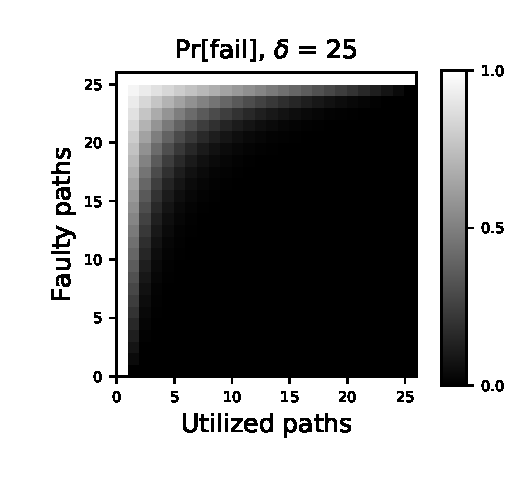
\includegraphics{fig-perror}}
\caption{
The probability of an undetectable error as a function of the number of
redundant channels and the number of adversarial faults.
\DIFaddbeginFL \DIFaddFL{A small increase in the number of utilized paths (network traffic)
can compensate for a large increase in attacker power.
}\DIFaddendFL }
\label{fig:pfail}
\end{figure}

\subsection*{Bounded Trust Model}

So far, we have assumed that Alice and Bob have access to some number
$\delta$ of channels with statistically independent faults.
However, in real communication architectures, direct links between all
pairs of individuals are not possible and messages must be routed through
a number of intermediate nodes.
In an adversarial setting,
the existence of intermediate nodes introduces two problems:
1. intermediate nodes may be compromised by the adversary and
2. faults on paths are no longer statistically independent:
two paths may pass through the same compromised node.
We show how to how to resolve these problems using a combination of network
structure and bounded trust transitivity.

Trust-based approaches to secure communication assume that some parties
cannot be compromised.
One common approach, the web of trust
\DIFdelbegin \DIFdel{\mbox{%DIFAUXCMD
\cite{zimmermann_official_1995,ferguson_practical_2003}}%DIFAUXCMD
,
extends trustinfinitely transitively:
Alice trusts her friends, as well as her friends' friends,
and so on}\DIFdelend \DIFaddbegin \DIFadd{\mbox{%DIFAUXCMD
\cite{zimmermann_official_1995,richters_trust_2011}}%DIFAUXCMD
.
Alice has }{\em \DIFadd{direct trust}} \DIFadd{for some number of nodes.
Alice has }{\em \DIFadd{indirect trust}} \DIFadd{for nodes separated by two or more hops of
direct trust.
Typically, this transitive trust is extended indefinitely,
sometimes reduced by a multiplicative factor at each step}\DIFaddend .
However, the assumption of infinitely transitive trust is unrealistic
\cite{christianson_why_1997}.
Furthermore, infinite trust transitivity obscures the importance of network structure,
as it depends only on whether some path exists, not the number or quality of paths.
\DIFdelbegin %DIFDELCMD < 

%DIFDELCMD < %%%
\DIFdel{An alternative assumption might be that each hop away from Alice in
in the network reduces the probability that a node can resist compromise
by a multiplicative constant.
Such a situation could occur if nodes more distant from Alice are
more favorably disposed to Alice's adversary, more likely to cooperate with that adversary, or less likely to take proactive security measures against that
adversary.
An even simpler version assumes that }\DIFdelend \DIFaddbegin \DIFadd{We adopt a simpler, yet more realistic }{\em \DIFadd{bounded trust}} \DIFadd{assumption:
that }\DIFaddend nodes up to some fixed number of hops cannot be compromised,
and that those beyond can.
This \DIFdelbegin \DIFdel{simplified version is still more realistic than infinite transitivity
and }\DIFdelend \DIFaddbegin \DIFadd{assumption }\DIFaddend will be convenient for proving our results\DIFdelbegin \DIFdel{.
We }\DIFdelend \DIFaddbegin \DIFadd{,
which we }\DIFaddend now proceed to define \DIFdelbegin \DIFdel{our model }\DIFdelend formally.

We define the {\em bounded trust model} on
an undirected graph $G = (V,E)$,
although the model can easily be extended to directed multigraphs.
Vertices representing communicating parties,
with edges representing mutually trusted communication links.
We define a {\em trust radius} $h$ such that nodes $v$ and
$w$ trust each other if their distance is less than $h$.
For a given node $v$,
we call the set of trusted nodes its
{\em trusted neighborhood} $T_h(v)$,
and all nodes at exactly distance $h$ the
{\em trust boundary} $B_h(v)$:
\beq
T_h(v) &=& \left\{ w \mid d(v,w) < h \right\} \\
B_h(v) &=& \left\{ w \mid d(v,w) = h \right\}.
\eeq
The trust boundary $B_h$ plays an important role because these nodes are not
trusted by $u$,
and if compromised can entirely isolate $v$ from the rest of the network.

Now let $s \in V$ be an arbitrary sender
and $t \in V$ be an arbitrary receiver.
We assume the presence of an adversary who knows the
full structure of the network,
and who can compromise a fixed number of nodes,
gaining complete control of their behavior.
We also assume that the adversary is specifically targeting communication
between $s$ and $t$ and
can compromise any node except for those trusted by $s$ or $t$.
Under these trust assumptions, adversarial faults can only occur
outside the trusted neighborhoods of $s$ and $t$:
$V \setminus \left(T_h(v) \cup T_h(w)\right)$.
We refer to this set of nodes as the {\em untrusted region}.
We now show how it is possible to communicate reliably,
even when all available paths go through the untrusted region.

\subsection*{Effective Redundancy}

Our approach is to achieve fault tolerance through redundancy.
To do so, we must use only
{\em independent paths} \cite{reiter_resilient_1998},
which have no common points of failure.
Typically, it is assumed that in order to be independent,
paths must be internally vertex disjoint, i.e.,
have no nodes in common except the endpoints.
However, under the bounded trust model,
intersecting paths can still be independent if their
intersection contains only trusted nodes.
We define two paths with common endpoints
to be {\em $h$-internally vertex disjoint}
if all common vertices are less than distance $h$ from
one of the endpoints.
This condition holds if and only if two paths are independent
under the bounded trust model with radius $h$.

When trust radius $h$ is assumed,
the number of $h$-internally vertex disjoint paths between
two nodes $s$ and $t$ represents the number of
channels that can be constructed between them having
statistically independent faults.
We thus refer to this quantity as the 
{\em effective redundancy} $\delta_{s,t,h}$.
The effective redundancy can also be interpreted as the
max-flow/min-cut of a graph after each trusted neighborhood has been
collapsed into a single vertex.
The trust boundaries form a cut of the network and place an upper bound on the
min-cut:
\beq
\delta_{v,w,h} \leq \min\left( \mid B_h(s) \mid, \mid B_h(t) \mid \right).
\eeq
Equality holds when there are no bottlenecks within the untrusted region,
an indication that the network is decentralized.
The effective redundancy of the entire graph can be characterized by the minimum
over all vertex pairs:
\beq
\delta_h(G) \equiv \min_{s,t \in V} \delta_{s,t,h}.
\eeq
Thus, for any pair of nodes in the network, at least $\delta_h$ independent,
redundant paths can be constructed between them.
The more quickly $\delta_h$ grows with $h$,
the better a network is at leveraging trust transitivity to create redundancy.
Thus, the scaling of $\delta_h$ can be used to quantify a network's ability
to withstand targeted attacks,
even when the exact trust radius $h$ is unknown.

\begin{figure}
\centerline{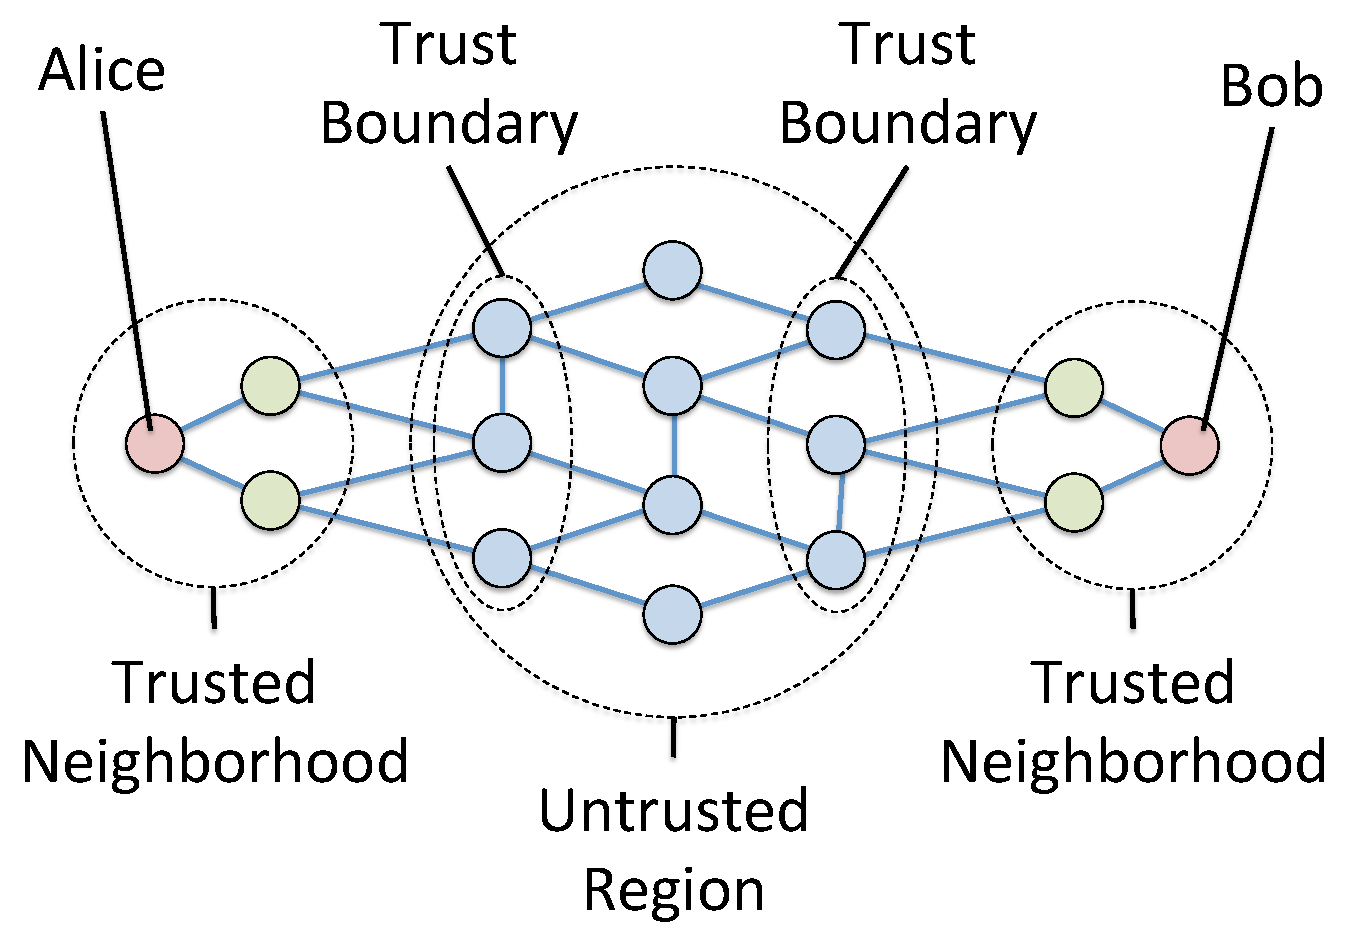
\includegraphics[width=4in,height=2.78in]{fig-partial-trust.pdf}}
\caption{
Illustration of a trusted communication network and the network properties
used by the {\em bounded trust model}.
Edges represent mutually trusted communication links.
The sender (Alice, $s$) and receiver (Bob, $t$) trust all nodes
less than the {\em trust radius} $h$ hops away.
These nodes form their {\em trusted neighborhoods} $T_h(v)$ and $T_h(w)$.
We assume that all faults occur in the remaining nodes: the
{\em untrusted region}.
The untrusted nodes in contact with the trusted neighborhoods for the
{\em trust boundaries} $B_h(v)$ and $B_h(w)$,
which (in the absence of central bottlenecks) determine the
{\em effective redundancy} $\delta_h$ provided by the network.
Alice and Bob can achieve the same level of attack-tolerance
as if they were directly connected by $\delta_h$ redundant channels.
}
\label{fig:trust-source}
\end{figure}

\subsection*{Structured Multipath Fault Tolerance}

Finding a maximal set of independent paths for an arbitrary network is NP hard
\cite{reiter_resilient_1998},
posing a challenge for multipath fault tolerance.
We propose side-stepping this problem by using structured networks,
for which independent paths can be generated efficiently.
We call this approach {\em structured multipath fault tolerance} (SMFT),
and now proceed to show how it is implemented on the butterfly
network topology.

\section*{The Butterfly Network Topology}
\label{sec-butterfly}

In order to implement structured multipath fault tolerance,
we need a structured network topology with high effective redundancy.
In this paper, we apply SMFT to the butterfly network topology
\cite{kshemkalyani_distributed_2008}.
The \DIFdelbegin \DIFdel{structure of the }\DIFdelend butterfly network is highly \DIFdelbegin \DIFdel{constrained}\DIFdelend \DIFaddbegin \DIFadd{structured}\DIFaddend ,
making it most suitable for applications where portions of the network structure
can be \DIFdelbegin \DIFdel{designed or dictated.
Examples of
such networks include:
overlay networks \mbox{%DIFAUXCMD
\cite{lua_survey_2005, korzun_structured_2013}}%DIFAUXCMD
,
formal organizations \mbox{%DIFAUXCMD
\cite{mohr_explaining_1982}}%DIFAUXCMD
,
government-regulated cellular networks \mbox{%DIFAUXCMD
\cite{walker_mass_2012}}%DIFAUXCMD
,
and call tree notification systems \mbox{%DIFAUXCMD
\cite{nickerson_thinking_2010}}%DIFAUXCMD
}\DIFdelend \DIFaddbegin \DIFadd{controlled or influenced.
The butterfly network is also recursive, with larger versions composed out of
multiple smaller versions,
making it possible for independently organized
attack-tolerant networks to merge into larger ones over time}\DIFaddend .
More flexible architectures may be possible,
but attack-tolerance will always require some level of influence over
network structure in order to limit single points of failure.
To address the case when the network cannot be fully controlled,
we show how partially rewiring a snapshot of the internet's router
network can greatly increase it's effective redundancy and
attack-tolerance properties\DIFaddbegin \DIFadd{, without requiring additional edges}\DIFaddend .

\subsection*{Butterfly Network Topology}

We choose the butterfly topology
\cite{kshemkalyani_distributed_2008}
because of several desirable properties (described below)
and because its structure allows for relatively straightforward
design and analysis of routing algorithms.
While several variations on the butterfly network exist,
we utilize the $m$-dimensional, directed wrap-around butterfly
(Fig. \ref{fig:bf-route}),
denoted $\wbf(m)$:
\beq
\wbf(m) &=& (V, E_\downarrow \cup E_\rightarrow) \\
V &=& \mathbb{Z}_{m} \times \mathbb{Z}_2^m \\
E_\downarrow
&=&
\{((l,z),(l+1 \; (\text{mod } m),z) \} \\
E_\rightarrow
&=&
\{(l,z),(l+1 \; (\text{mod } m),
z \oplus 1_l \},
\eeq
where $\mathbb{Z}_m$ is the set of integers modulo $m$,
$\oplus$ represents component-wise addition modulo 2,
and $1_l$ is a vector with a 1 in index $l$ and 0 elsewhere.
Each node is associated with a level $l$ and an $m$-bit string $z$
known as {\em the place-within-level}.
There are two types of edges: down, and down-right
(shown in Fig. \ref{fig:butterfly}).
Down edges ($E_\downarrow$) connect nodes sharing the same $z$ value
in a cycle of increasing level $l$.
Down-right edges ($E_\rightarrow$) also link to a node of level $l + 1$,
but one having the place-within-level equal to $z$ with the $l$th bit inverted.

\begin{figure}[!h]
\begin{center}
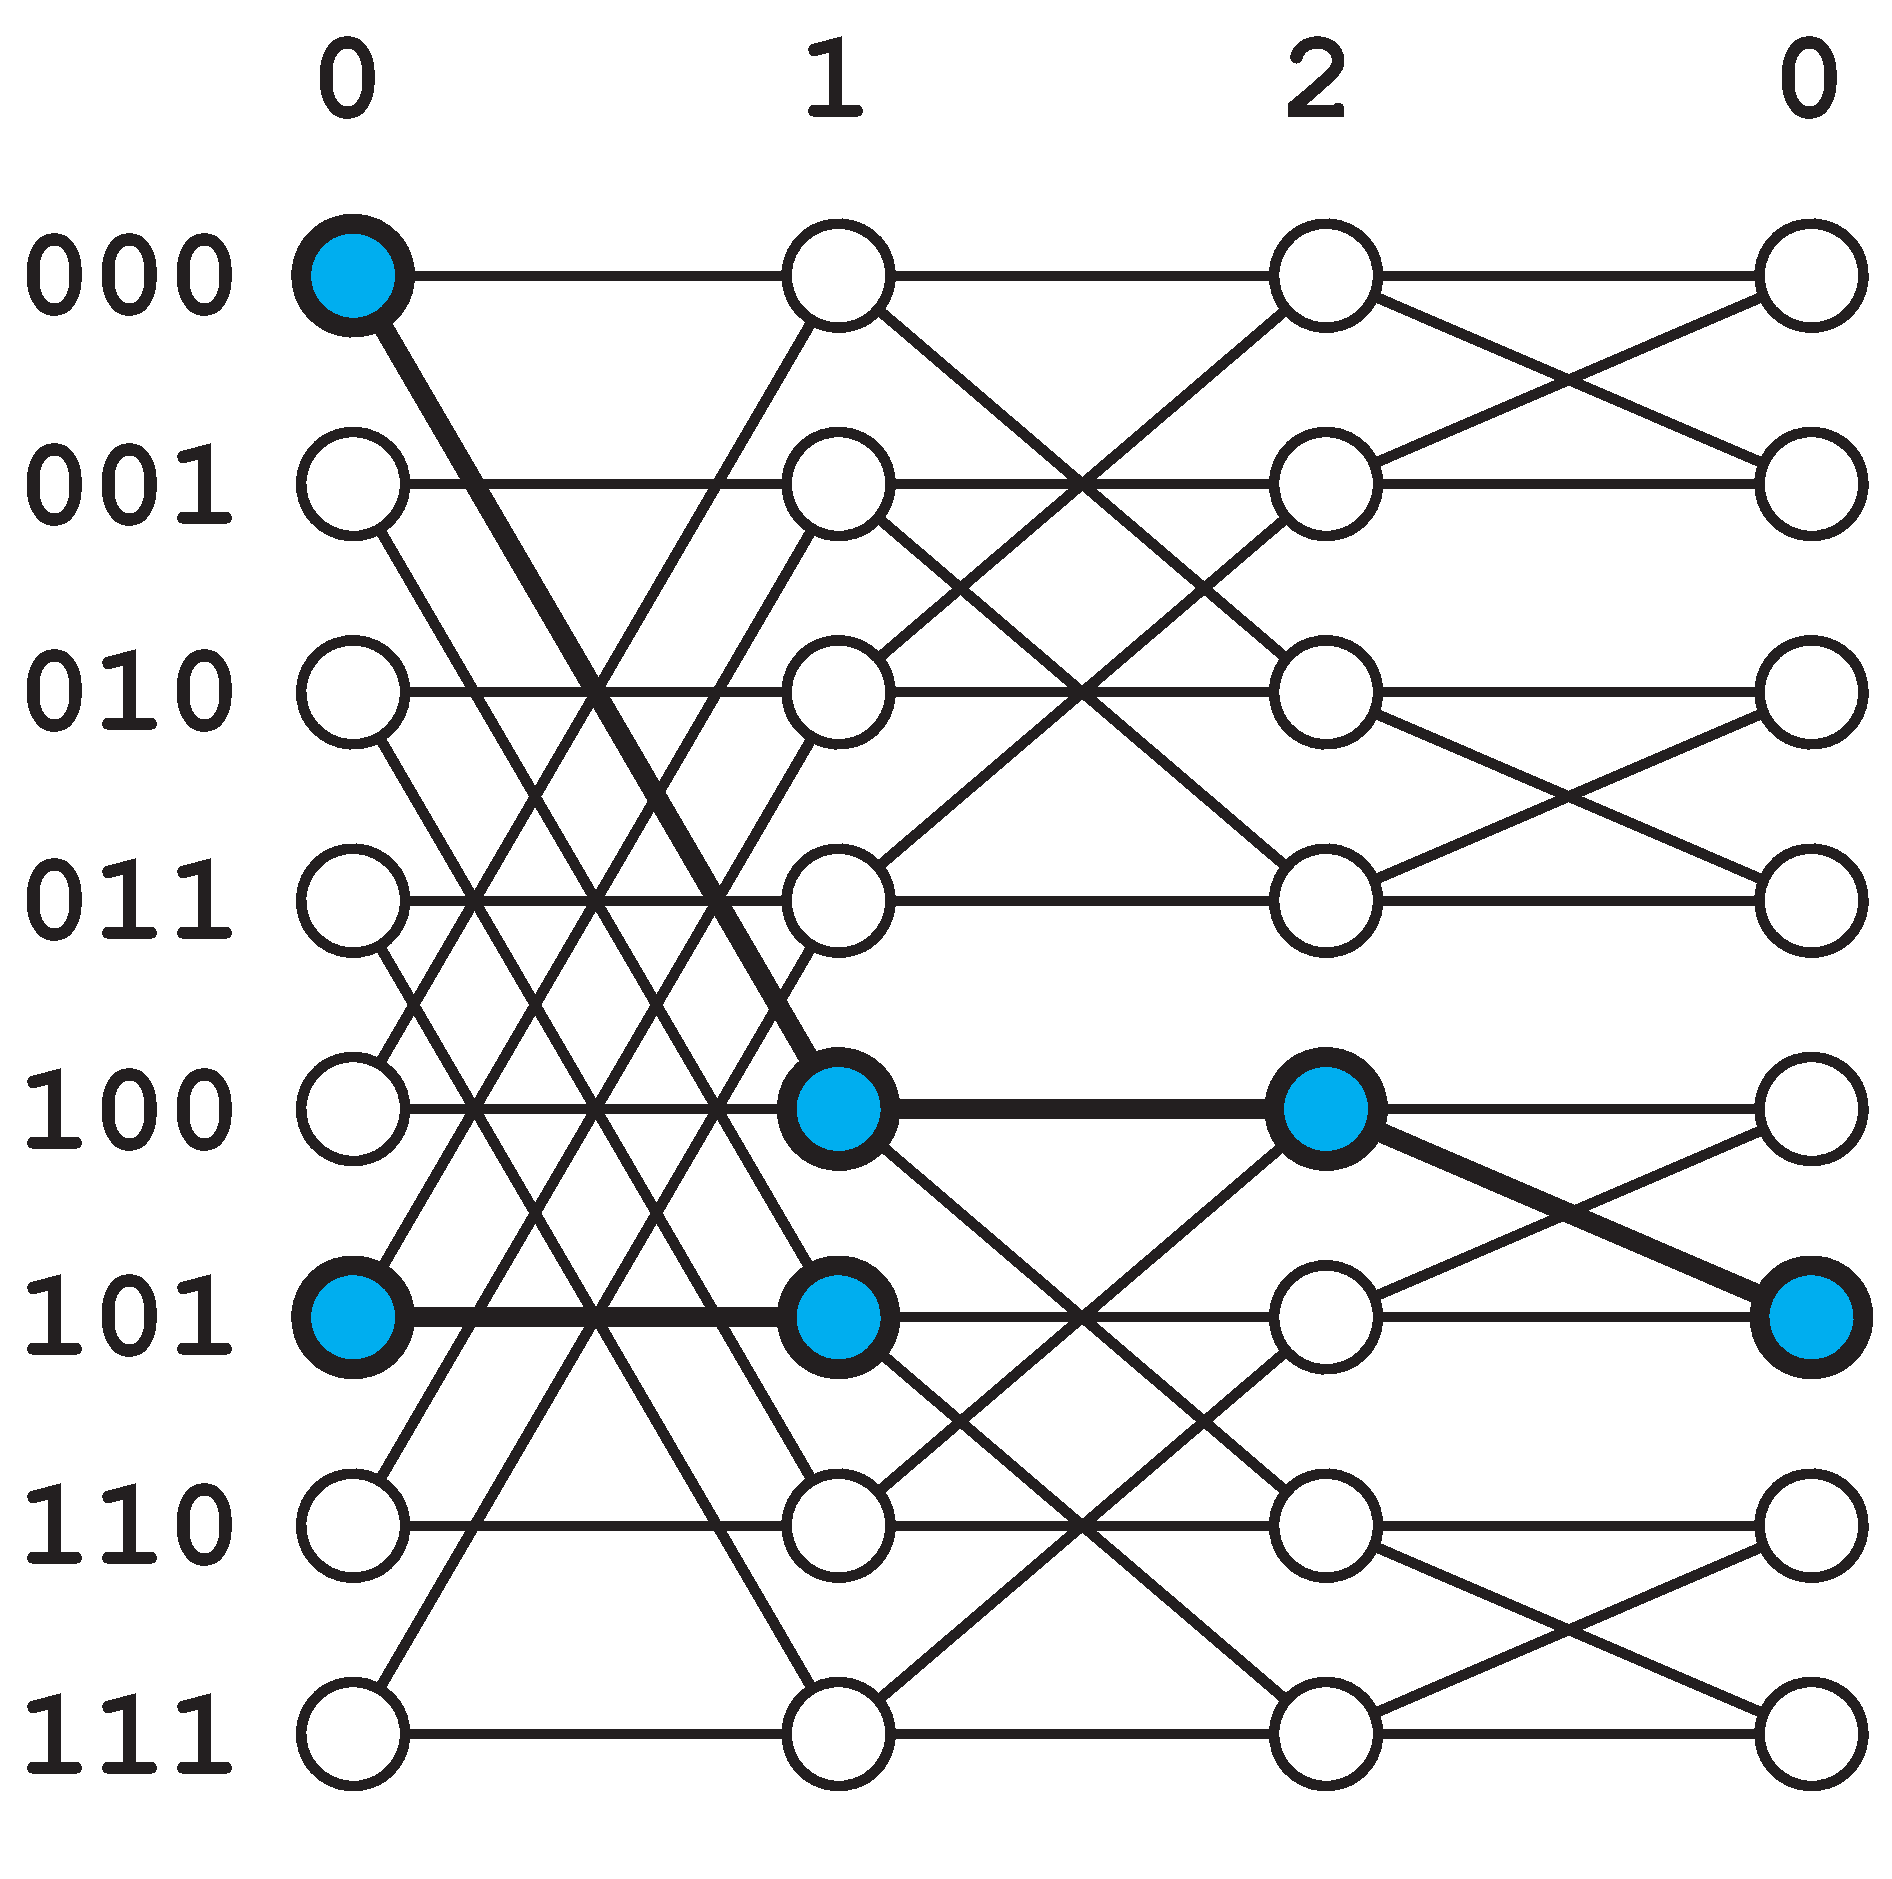
\includegraphics[height=3in]{fig-bf-route}
\end{center}
\caption{
A 3-dimensional wraparound butterfly network.
Note that the rightmost nodes are the same nodes as the leftmost,
drawn twice for visual clarity.
The highlighted nodes and edges show the path from node (0,000)
to node (1,101).
\label{fig:bf-route}
}
\end{figure}

\begin{figure}[!h]
\begin{center}
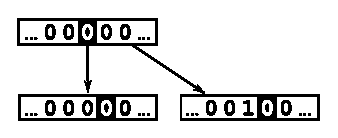
\includegraphics{fig-butterfly}
\end{center}
\caption{
Schematic illustration of the two types of edges in a directed butterfly
network.
The node $(l,z)$ is shown as the bit string $z$ with a square around the
$l$th bit.
``Down'' edges increment $l$, leaving $z$ unchanged,
while ``down-right'' edges increment $l$ and invert the $l$th bit of $z$.
In the wrap-around variant, the nodes with maximum $l$ have down and down-right
edges to the nodes with $l=0$.
\label{fig:butterfly}
}
\end{figure}

The wrap-around butterfly network is known to have several of the properties
we desire for scalable, decentralized communication networks:
 \begin{description} 
\item[Vertex-transitivity:]
Because the wrap-around butterfly is vertex transitive,
it is maximally decentralized;
\item[Small-diameter:]
For any two nodes, the length of the shortest path between them is
$O(\log N)$, where N is the number of nodes in the network
\DIFaddbegin \DIFadd{(corresponding to low-latency in real-world terms)}\DIFaddend ;
\item[Sparsity:]
With a constant degree of 4, the wrap-around butterfly is extremely sparse,
and can scale indefinitely without node degree becoming a limitation;
\item [Redundancy:]
Multiple paths exist between any two nodes.
Specifically, we will prove below that the number of
$h$-internally vertex disjoint paths between two
nodes increases exponentially with $h$.
 \end{description} 

The structure of the butterfly network lends itself to a well-known
(unipath) routing algorithm (Fig. \ref{fig:bf-route}),
which we later extend to the multipath case.
The unipath algorithm first follows a down or down-right edge at every step,
increasing the level $l$ by 1 and cycling through the
indices of the place-within-level.
If the current node's place-within-level matches the destination node's at
index $l$,
a down edge is chosen and the place-within-level does not change.
Otherwise, a down-right edge is chosen and the $l$th component of the
place-within-level is flipped,
after which it matches the destination.
After $m$ iterations of this, all levels have been visited
and the place-within-level matches that of the destination.
Simply following down (or up) edges will then increment (decrement) the
level until the destination node is reached.

\subsection*{Butterfly Rewiring}

Even when a butterfly topology cannot be implemented perfectly,
it can still increase the attack tolerance properties of a network.
Here, we simulate targeted attacks against a snapshot of the internet's
router network on January 2, 2000
\cite{leskovec_graphs_2005}, having 6493 nodes and 13914 edges.
At each step of the simulation, betweenness centrality is recalculated and the
most central node is removed.
We also simulate attack on several rewired networks.
\DIFaddbegin \DIFadd{The rewiring process alters the network structure to resemble a butterfly
topology, without adding any additional edges.
}\DIFaddend We 1. generate edges corresponding to a 9-dimensional butterfly network between
the 4608 highest-degree router nodes,
2. choose a fraction $f$ of those edges at random,
3. add those edges to the router network, and
4. remove an equal number of the original edges at random.

Our simulations show improved resistance to fragmentation and higher
effective redundancy when even a fraction of edges have been rewired to
match the butterfly topology.
While the original router network fragments when about 1\% of the nodes
have been removed (Fig. \ref{fig:diameter}),
this number increases to 2\%
with only 10\% of the butterfly edges present.
With 90\% of the butterfly edges present
the network remains unfragmented beyond the failure of the 8\% most
central nodes.
The effective redundancy for various values of trust transitivity $h$
are shown in Fig. \ref{fig:mincut}.
The effective redundancy is calculated by collapsing nodes and edges within
$h$ hops of source and destination into single nodes and finding the min-cut
between them,
averaging over 150 source-destination pairs.
For $h=0$, the rewired version has strictly higher redundancy.
For $h>0$,
the original network has higher redundancy when the number of failures is small,
while the rewired network has higher redundancy beyond a crossover point.
We interpret these results to suggest that even when a small number of
highly central nodes have been removed from a heavy-tailed network,
most nodes are still able to take advantage of the remaining hubs.
As larger hubs continue to be removed, the connectivity of the network
decreases until the crossover point,
at which point the rewired network offers higher effective redundancy.

\begin{figure}
\centerline{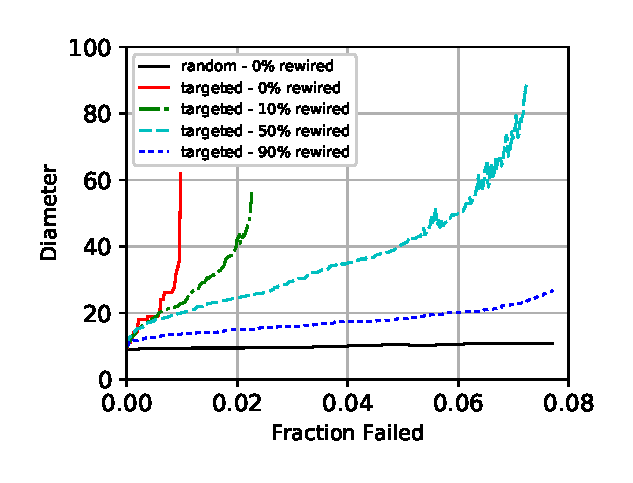
\includegraphics{fig-diameter}}
\caption{
Simulation of targeted attacks against a snapshot of the internet's router
network with a fraction of the edges rewired into a partial butterfly configuration.
The original network fragments \DIFdelbeginFL \DIFdelFL{at about }\DIFdelendFL \DIFaddbeginFL \DIFaddFL{when the top }\DIFaddendFL 1\% \DIFaddbeginFL \DIFaddFL{of nodes are removed}\DIFaddendFL .
With \DIFdelbeginFL \DIFdelFL{90}\DIFdelendFL \DIFaddbeginFL \DIFaddFL{only 10}\DIFaddendFL \% of the butterfly edges present,
\DIFaddbeginFL \DIFaddFL{this value doubles to 2\%.
With 90\% of }\DIFaddendFL the \DIFaddbeginFL \DIFaddFL{edtges rewired,
the }\DIFaddendFL network remains unfragmented beyond the failure of the 8\% most
central nodes.
\DIFaddbeginFL \DIFaddFL{The rewiring scheme does not require adding any additional edges.
}\DIFaddendFL }
\label{fig:diameter}
\end{figure}

\begin{figure*}[h!]
\centerline{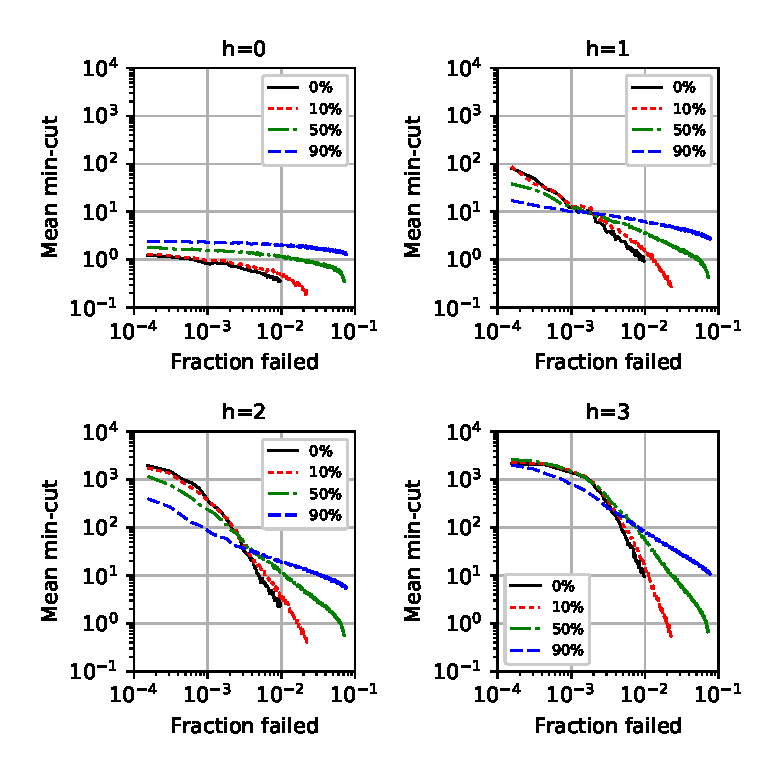
\includegraphics[width=5in,height=5in]{fig-mincut}}
\caption{
Simulation of targeted attacks against a snapshot of the internet's router
network with a fraction of the edges rewired into a partial butterfly configuration.
The effective redundancy is shown for several values of trust transitivity $h$.
For $h>0$, the original network has higher effective redundancy up to a crossover point,
after which the rewired network performs better.
}
\label{fig:mincut}
\end{figure*}

\section*{Multipath Butterfly Routing}
\label{sec-bf-route}

We now present a routing algorithm to construct $2^h$ independent paths
between two nodes in a butterfly network,
where $h$ is the trust radius under the partial trust model.
Informally, Alice sends each message to a distinct node on her
trust boundary, then to a distinct intermediate node in the untrusted region,
then to a distinct node on Bob's trust boundary, and finally to Bob.
The intermediate nodes are in a sense ``far'' from each other and ensure that
no two paths overlap in the untrusted region.
Each path can be parameterized by a single integer $s$, which identifies
the specific node on Alice's trust boundary
(or equivalently the node on Bob's trust boundary, or the untrusted intermediate).

The algorithm guarantees paths are independent by ensuring that
(outside the trusted neighborhoods)
they only include
nodes that match the path parameter $s$ at certain indexes in their
place-within-level.
Since each path has a unique parameter $s$,
its set of untrusted nodes is disjoint from all other paths.
As with the unipath routing algorithm,
each of the multiple paths proceed from a source $v$ to a destination $u$
using down and down-right edges,
cycling through levels one at a time.
However, we cycle through the levels twice, once to route from $v$ to a
particular path's intermediary node,
and again to route from the intermediary to $w$.
Each cycle is divided into stages,
with different properties used to prove independence at each stage
(see Fig. \ref{fig:route-overview}).
In the first cycle (stages 1--4), path independence is guaranteed by ensuring that
all nodes match the path parameter $s$ in the first $h$ bits of the place-within-level.
Similarly, in the second cycle (stages 5--7),
independence is guaranteed by ensuring that all paths match $s$ in the
$h$ bits of the place-within-level preceding the destination index.
A full example is illustrated in Fig. \ref{fig:routing}.

\begin{table}[h!]
\caption{Butterfly Multipath Routing Variables\label{tab:routing}}
\begin{center}
\DIFdelbeginFL %DIFDELCMD < \begin{tabular}{|l|l|}
%DIFDELCMD < \hline
%DIFDELCMD < %%%
\DIFdelFL{NAME }\DIFdelendFL \DIFaddbeginFL \begin{tabular}{ll}
\DIFaddFL{Name }\DIFaddendFL & \DIFdelbeginFL \DIFdelFL{VARIABLE }\DIFdelendFL \DIFaddbeginFL \DIFaddFL{Variable }\DIFaddendFL \\\hline
butterfly dimension & $m \in \mathbb{Z}_+$ \\
\DIFdelbeginFL %DIFDELCMD < \hline
%DIFDELCMD < %%%
\DIFdelendFL node level & $l \in \mathbb{Z} : 0 \leq l < m$ \\
\DIFdelbeginFL %DIFDELCMD < \hline
%DIFDELCMD < %%%
\DIFdelendFL node place within level & $z \in \mathbb{Z}_2^m$ \\
\DIFdelbeginFL %DIFDELCMD < \hline
%DIFDELCMD < %%%
\DIFdelendFL trust radius & $h \in \mathbb{Z} : 1 \leq h \leq \lfloor m/2 \rfloor$ \\
\DIFdelbeginFL %DIFDELCMD < \hline
%DIFDELCMD < %%%
\DIFdelendFL path index & $s \in \mathbb{Z}_2^h$ \\
\DIFdelbeginFL %DIFDELCMD < \hline
%DIFDELCMD < %%%
\DIFdelendFL \end{tabular}
\end{center}
\end{table}

\begin{figure}[h!]
\begin{center}
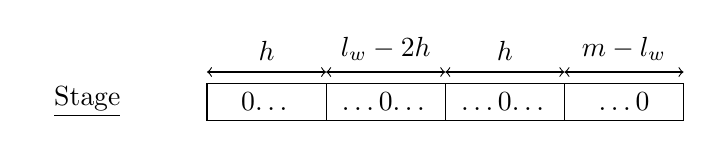
\begin{tikzpicture}[
node distance=0pt,
 start chain = A going right,
    X/.style = {rectangle, draw,% styles of nodes in string (chain)
                minimum width=10ex, minimum height=3ex,
                outer sep=0pt, on chain},
                        ]
\foreach \i in {0\ldots,{\ldots}0\ldots,{\ldots}0\ldots,{\ldots}0}% <-- content of nodes
    \node[X] {\i};
\draw[<->] ([yshift=1.5mm] A-1.north east) -- node[above=0.25mm] {$h$} ([yshift=1.5mm] A-1.north west);
\draw[<->] ([yshift=1.5mm] A-2.north east) -- node[above=0.25mm] {$l_w - 2h$} ([yshift=1.5mm] A-2.north west);
\draw[<->] ([yshift=1.5mm] A-3.north east) -- node[above=0.25mm] {$h$} ([yshift=1.5mm] A-3.north west);
\draw[<->] ([yshift=1.5mm] A-4.north east) -- node[above=0.25mm] {$m - l_w$} ([yshift=1.5mm] A-4.north west);
\draw ( A-1.west) -- node[left=5ex,minimum width=10ex] {\underline{Stage}} ( A-1.west);
\end{tikzpicture}
\\
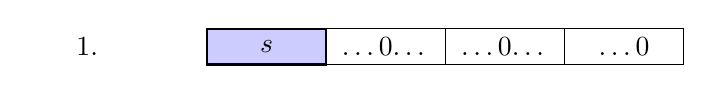
\begin{tikzpicture}[
node distance=0pt,
 start chain = A going right,
    X/.style = {rectangle, draw,% styles of nodes in string (chain)
                minimum width=10ex, minimum height=3ex,
                outer sep=0pt, on chain},
    Y/.style = {rectangle, draw,% styles of nodes in string (chain)
                minimum width=10ex, minimum height=3ex,
                outer sep=0pt, on chain, thick, fill=blue!20!white},
                        ]
\node[Y] {$s$};
\foreach \i in {{\ldots}0\ldots,{\ldots}0\ldots,{\ldots}0}% <-- content of nodes
    \node[X] {\i};
\draw ( A-1.west) -- node[left=5ex,minimum width=10ex] {1.} ( A-1.west);
\end{tikzpicture}
\\
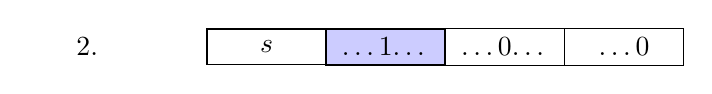
\begin{tikzpicture}[
node distance=0pt,
 start chain = A going right,
    X/.style = {rectangle, draw,% styles of nodes in string (chain)
                minimum width=10ex, minimum height=3ex,
                outer sep=0pt, on chain},
    Y/.style = {rectangle, draw,% styles of nodes in string (chain)
                minimum width=10ex, minimum height=3ex,
                outer sep=0pt, on chain, thick, fill=blue!20!white},
                        ]
\foreach \i in {$s$}% <-- content of nodes
    \node[X] {\i};
\node[Y] {{\ldots}1\ldots};
\foreach \i in {{\ldots}0\ldots,{\ldots}0}% <-- content of nodes
    \node[X] {\i};
\draw ( A-1.west) -- node[left=5ex,minimum width=10ex] {2.} ( A-1.west);
\end{tikzpicture}
\\
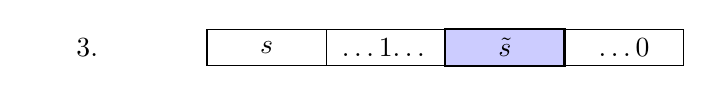
\begin{tikzpicture}[
node distance=0pt,
 start chain = A going right,
    X/.style = {rectangle, draw,% styles of nodes in string (chain)
                minimum width=10ex, minimum height=3ex,
                outer sep=0pt, on chain},
    Y/.style = {rectangle, draw,% styles of nodes in string (chain)
                minimum width=10ex, minimum height=3ex,
                outer sep=0pt, on chain, thick, fill=blue!20!white},
                        ]
\foreach \i in {$s$,{\ldots}1\ldots}% <-- content of nodes
    \node[X] {\i};
\node[Y] {$\tilde{s}$};
\foreach \i in {{\ldots}0}% <-- content of nodes
    \node[X] {\i};
\draw ( A-1.west) -- node[left=5ex,minimum width=10ex] {3.} ( A-1.west);
\end{tikzpicture}
\\
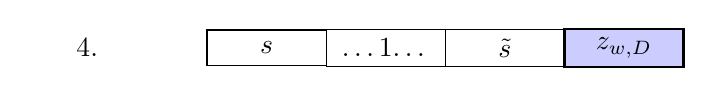
\begin{tikzpicture}[
node distance=0pt,
 start chain = A going right,
    X/.style = {anchor=base, rectangle, draw,% styles of nodes in string (chain)
                minimum width=10ex, minimum height=3ex,
                outer sep=0pt, on chain},
    Y/.style = {rectangle, draw,% styles of nodes in string (chain)
                minimum width=10ex, minimum height=3ex,
                outer sep=0pt, on chain, thick, fill=blue!20!white},
                        ]
\foreach \i in {$s$,{\ldots}1\ldots,$\tilde{s}$}% <-- content of nodes
    \node[X] {\i};
\node[Y] {$z_{w,D}$};
\draw ( A-1.west) -- node[left=5ex,minimum width=10ex] {4.} ( A-1.west);
\end{tikzpicture}
\\
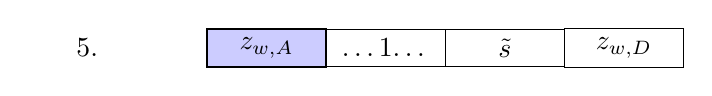
\begin{tikzpicture}[
node distance=0pt,
 start chain = A going right,
    X/.style = {anchor=base, rectangle, draw,% styles of nodes in string (chain)
                minimum width=10ex, minimum height=3ex,
                outer sep=0pt, on chain},
    Y/.style = {rectangle, draw,% styles of nodes in string (chain)
                minimum width=10ex, minimum height=3ex,
                outer sep=0pt, on chain, thick, fill=blue!20!white},
                        ]
\node[Y] {$z_{w,A}$};
\foreach \i in {{\ldots}1\ldots,$\tilde{s}$,$z_{w,D}$}% <-- content of nodes
    \node[X] {\i};
\draw ( A-1.west) -- node[left=5ex,minimum width=10ex] {5.} ( A-1.west);
\end{tikzpicture}
\\
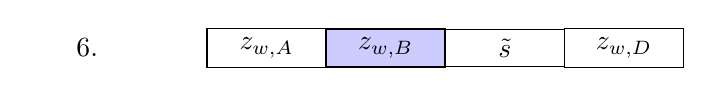
\begin{tikzpicture}[
node distance=0pt,
 start chain = A going right,
    X/.style = {anchor=base, rectangle, draw,% styles of nodes in string (chain)
                minimum width=10ex, minimum height=3ex,
                outer sep=0pt, on chain},
    Y/.style = {rectangle, draw,% styles of nodes in string (chain)
                minimum width=10ex, minimum height=3ex,
                outer sep=0pt, on chain, thick, fill=blue!20!white},
                        ]
\foreach \i in {$z_{w,A}$}% <-- content of nodes
    \node[X] {\i};
\node[Y] {$z_{w,B}$};
\foreach \i in {$\tilde{s}$,$z_{w,D}$}% <-- content of nodes
    \node[X] {\i};
\draw ( A-1.west) -- node[left=5ex,minimum width=10ex] {6.} ( A-1.west);
\end{tikzpicture}
\\
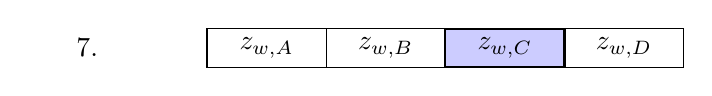
\begin{tikzpicture}[
node distance=0pt,
 start chain = A going right,
    X/.style = {anchor=base, rectangle, draw,% styles of nodes in string (chain)
                minimum width=10ex, minimum height=3ex,
                outer sep=0pt, on chain},
    Y/.style = {rectangle, draw,% styles of nodes in string (chain)
                minimum width=10ex, minimum height=3ex,
                outer sep=0pt, on chain, thick, fill=blue!20!white},
                        ]
\foreach \i in {$z_{w,A}$,$z_{w,B}$}% <-- content of nodes
    \node[X] {\i};
\node[Y] {$z_{w,C}$};
\foreach \i in {$z_{w,D}$}% <-- content of nodes
    \node[X] {\i};
\draw ( A-1.west) -- node[left=5ex,minimum width=10ex] {7.} ( A-1.west);
\end{tikzpicture}
\end{center}
\caption{
Progression of place-within-level $z$ as the multipath routing algorithm
cycles through the levels of the butterfly network.
\label{fig:route-overview}
}
\end{figure}

\begin{figure}[!h]
\begin{center}
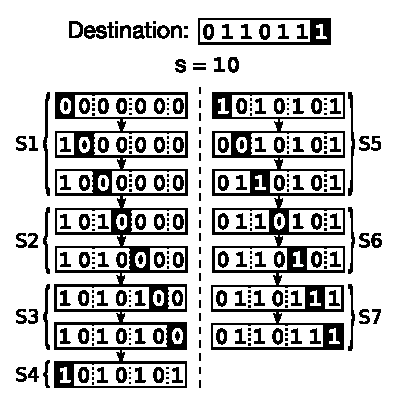
\includegraphics{fig-routing}
\end{center}
\caption{
An example of one path as constructed by the proposed multipath
routing algorithm.
The path is shown for $s = 10_2$
and $w = (6, 0110111_2)$.
\label{fig:routing}
}
\end{figure}

\subsection*{Algorithm Specification}

We now begin the formal specification of our multipath routing scheme for the
wrap-around butterfly network.
For convenience, the relevant variables are summarized in Table \ref{tab:routing}.
Utilizing vertex transitivity, we label the source node as
$(l^{(0)}, z^{(0)}) = (0, 0)$ and denote the destination node as $w = (l_w, z_w)$,
without loss of generality.

Let $s$ be an $h$-bit binary string with $s_i$ denoting the bit at index $i$.
There are $2^h$ such strings.
Let $v_s^{(t)} = (l^{(t)}, z^{(t)})$ be the node at position $t$
in the path parameterized by $s$.
For convenience,
we will omit the subscript $s$ when it is obvious from context.
We define three distinct partitions of $m$-bit binary strings.
Let $Q_{v^{(0)}}$ be the set of $m$-bit
strings in which the bits at
all indices $h \leq i < l_w - h$ match those of $z^{(0)}$,
and let $\overline{Q_{v^{(0)}}}$ be its complement.
Note that $Q_{v^{(0)}}$ is trivially all $m$-bit strings if $l_w < 2h$.
Let $R_s$ be the set of $m$-bit strings with the lowest $h$
bits all matching the bits of $s$,
and let $\overline{R_s}$ be its complement.
Let $S_s$ be the set of $m$-bit strings with the $h$ bits
preceding index $l_w$ all matching the bits of $\tilde{s}$,
where $\tilde{s}$ is a cyclic permutation of $s$:
\beq
\tilde{s}_i &=& s_{(i + l_w) \text{ mod } h},
\eeq
and let $\overline{S_s}$ be its complement.
We will make use of the fact that:
\beq
s \neq s^\prime &\implies&
S_s \cap S_{s^\prime} = R_s \cap R_{s^\prime} = \emptyset.
\eeq

Routes are constructed in 7 stages.
The network topology dictates that $l^{(t+1)} = l^{(t)} + 1$ (mod $m$),
so we let $l = t$ (mod $m$).
and that $z^{(t+1)}$ is equal to $z^{(t)}$ with or without the bit in index
$l^{(t)}$ inverted, depending on whether the down or down-right edge was
taken at step $t$.
 \begin{description} 
\item[Stage 1: ($0 \leq t < h$)]{
Down or down-right edges
are chosen such that the $t$th bit of $z^{(t+1)}$ is equal to the $t$th bit
of $s$.
Throughout Stage 1, all nodes are within the sender's trusted neighborhood.
Throughout Stage 1, $z^{(t)} \in Q_{v^{(0)}}$.
At the end of Stage 1, $z^{(h)} \in S_s$, and $z^{(t)}$ will remain so until the level cycles to $0$ at $t = m$.
}
\item[Stage 2: ($h \leq t < l_w - h$)]{
Edges are chosen to make the $t$th bit of
$z^{(t+1)}$ the inverse of the $t$th bit of $z^{(0)}$.
Note that this stage does not occur when $l_w < 2h$.
If this stage occurs, then $z^{(t)} \in \overline{Q_{v^{(0)}}}$ until these
levels are reached again in stage 6.
}
\item[Stage 3: ($l_w - h \leq t < l_w$)]{
The bits of $z^{(t)}$ are chosen to match $\tilde{s}$,
such that after the stage is complete, $z^{(t)} \in R_s$.
}
\item[Stage 4: ($l_w \leq t < m$)]{
Paths are chosen such that the $t$th bit of $z^{(t+1)}$ matches that of the
destination node $z_w$.
This stage will not occur if $l_w > m - h$.
}
\item[Stage 5: ($m \leq t < m + h$)]{
There are two cases.
If $2h < l_w < m - h$,
then there is no overlap between the indices defining $R_s$ and $S_s$.
In this case, the first $h$ bits of $z^{(t)}$ are set to
match $z_w$.
Otherwise there is some overlap between the indices defining $R_s$ and
$S_s$.
In this case, the each of the first $h$ bits of $z^{(t)}$ is either kept the
same if $l_w - h \leq l < l_w$, or set to the corresponding bit of $z_w$
otherwise.
In this stage and after, $z^{(t)}$ is no longer guaranteed to be in $R_s$.
However, $z^{(t)}$ remains in $S_s$ during and after this stage.
}
\item[Stage 6: ($m + h \leq t < m + l_w - h$)]{
In this stage, edges are chosen to set the bits of $z^{(t)}$ to their
corresponding value in $z_w$.
$z^{(t)} \in \overline{Q_{v^{(0)}}}$ throughout this stage,
but not afterwards.
}
\item[Stage 7: ($m + l_w - h \leq t < m + l_w$)] {
The $h$ bits of $z^{(t)}$
preceding index $l_w$ are set to match $z_w$.
All nodes in this stage are within $h$ hops of $w$ and thus in its trusted
neighborhood.
After this stage, $v^{(m + l_w)} = w$ and routing is complete.
}
 \end{description} 

\subsection*{Proof of Path Independence}

\begin{theorem}
Given an $m$-bit wrap-around butterfly network ($m > 1$),
and an integer $h$ ($1 \leq h \leq \left\lfloor \frac{m}{2} \right\rfloor$),
for all node pairs $(v, w)$ such that $d(v,w) \geq 2h$,
there exist at least $2^h$ $h$-internally vertex disjoint
paths $v_s$ ($0 \le s < 2^h$) from
$v$ to $w$ such that
$s \neq s^\prime \implies v_s \cap v_{s^\prime} \subset T_h(u) \cup T_h(v)$.
\end{theorem}
\begin{proof}
Nodes from two paths can only coincide if their levels are the same.
Nodes which share a level must either be in the same stage, or 4 stages
apart.
Let ($a$,$a^\prime$) denote a pair of sub-paths corresponding to stage $a$ of
one path and stage $a^\prime$ of another.
Excluding paths that intersect in their trusted neighborhoods, (1,1) and (7,7),
we have reduced the list of possible intersections to the following cases:
(2,2), (3,3), (4,4), (5,5), (6,6), (1,5), (2,6), and (3,7).
Nodes in stages 2--4 belong to $R_s$ so cannot overlap with any stage 2--4
nodes from another path, eliminating (2,2), (3,3), and (4,4).
Similarly, nodes in stages 4--6 belong to a unique $S_s$,
eliminating (5,5) and (6,6).
Nodes in stage 1 belong to $Q_{v^{(0)}}$ while those in stage 5 belong in
its complement, eliminating (1,5).
Similarly, for all $l$ in stage 2, $z^{(l)}$ is equal to $z^{(0)}$,
while in stage 6, $z^{(l)}$ is the inverse, eliminating (2,6)
This leaves only (3,7), a collision which can occur only for only one path
(with $s$ matching the first $h$ bits of $z_w$), and which enters the trusted
neighborhood in stage 3.
For this single path, we can proceed directly from stage 2 to stage 7,
eliminating the last possible collision.
\end{proof}

Thus, assuming the partial trust model with trust transitive
for $h$ hops, we can construct $2^h$ paths on a wrap-around butterfly topology
which do not intersect outside the trusted neighborhoods of the source and
destination.
Note that the node sequence $v_s^{(t)}$ can be calculated entirely
from the source $v$, destination $w$, and path parameter $s$,
meaning that with this information nodes are able to determine which neighbor
to route a given message copy to.
Furthermore, the existence of $2^h$ paths places a lower bound on the
effective redundancy $\delta_h$,
showing that the decentralized, redundant, structured networks such as the
butterfly can have a very low probability of failure when faced with
adversarial faults, even from a very powerful attacker.

\section*{Discussion}
\label{sec-discussion}

Our work has been motivated by the vulnerability of current communications
infrastructure to surveillance and censorship,
which are often achieved by coercive targeted attacks against central nodes.
We have already discussed two such cases:
Pakistan's inadvertant censorship of YouTube
\cite{hunter_pakistan_2008}
and the FBI's \DIFdelbegin \DIFdel{surveillance-turned-censorship }\DIFdelend \DIFaddbegin \DIFadd{surveillance and censorship }\DIFaddend of Lavabit
\cite{poulsen_edward_2013}.

\DIFaddbegin 

\DIFaddend The reader may wonder how our methods could be employed in scenarios
such as large-scale state-sponsored censorship
\cite{xu_internet_2011}.
Censorship-resistant infrastructure often replaces central servers
(e.g., the router in the 2008 YouTube incident) with multiple servers across
the world, synchronized through consensus protocols.
The {\em directory authorities} used by the Tor project
\cite{dingledine_tor:_2004} are one example.
However, the size of such networks is limited by the number of
trusted relationships (degree) each node can maintain, and the inherent insecurity of
extending transitive trust to an ever-larger network.
Our work provides both a theoretical framework
and a specific example of how network structure
can be engineered to leverage trust for a high level of attack-tolerance,
without sacrificing scalability.

We have focused primarily on adversarial faults that block or
change messages (censorship) but our work is also relevant to
surveillance.
While cryptographic anti-surveillance techniques exist,
they remain vulnerable to man-in-the-middle attacks,
in which an intermediate node masquerades as the destination.
Such attacks can be detected if the original message reaches the true
destination unaltered,
which SMFT can help to ensure.

In its current form, our work has several limitations.
Most obviously, it requires complete control over the network structure.
However, we have shown that even partially control over network structure can
improve attack tolerance properties.
Still a more flexible network structure is desirable.
There is also the question of how to construct such a network without a central
authority.
This limitation may not be as severe as it seems,
due to the nested structure of the butterfly network.
We conjecture that smaller independently-formed networks could be
merged into a single larger network without central coordination.
\DIFaddbegin \DIFadd{When nodes and edges exist in geographic space (as in cables connecting internet
routers) this scheme might require connections between very distant locations.
Such connections are extremely expensive to construct and maintain,
although many exist today in the form of redundant internet backbones and
undersea cables. An alternative solution might involve satellite links,
which connect distant geographic points much more easily.
While turning our network theoretical results into practical applications
will require considerable additional work, we believe that work is inevitably
necessary in order to create attack-tolerant networks.
}\DIFaddend 

In addition to addressing the above limitations,
we see several potential directions for future work.
The development of new structured networks or multipath routing algorithms
could achieve higher levels of redundancy and attack-tolerance.
It is also desirable to examine how changes to social dynamics could shift
self-organized networks towards a more decentralized structure.
Finally, our results could be implemented to address specific applications, e.g.,
secure messaging, domain name resolution, or anonymous web browsing.

\section*{Conclusion}
\label{sec-conclusion}

Coercion-resistant, topological approaches to attack tolerance are needed to
address the current vulnerability of communications infrastructure to
censorship and surveillance.
We have presented a novel concurrent multipath routing (CMR)
algorithm for the butterfly network,
as well as a structured multipath fault tolerance (SMFT) scheme,
which can be combined to create a coercion-resistant,
attack-tolerant point-to-point communication architecture.
We have also shown how assuming bounded trust
transitivity can enable a quantitative analysis of the
relationships between network structure, trust, and attack-tolerance.
In our architecture,
the probability of an adversary causing an undetectable error
decreases exponentially with the network's effective redundancy.
The effective redundancy, in the case of the butterfly topology,
grows exponentially with the radius of trust transitivity.
Furthermore, a small increase in the number of messages sent
\DIFaddbegin \DIFadd{(traffic volume) }\DIFaddend can compensate
for a large increase in the number of messages compromised by an adversary.
These results \DIFdelbegin \DIFdel{are directly applicable to systems in which the link
structure can be imposed by the designer}\DIFdelend \DIFaddbegin \DIFadd{require some control over the structure of a network,
or some portion of the network}\DIFaddend .
Even when network structure cannot be perfectly controlled,
we have shown that partially rewiring a snapshot of the internet's router network
can greatly increase its attack-tolerance properties.
We believe that this work provides a foundation for the
development of additional topology-based communication
architectures to guard against technical and coercive adversarial attacks,
including censorship and surveillance.

\section*{Acknowledgments}
The authors would like to thank Tony Garnock-Jones, A. Frederick Dudley, and
Nathaniel Bezanson for helpful conversations.
This research was partly supported by the National Science Foundation under
Grant No. IIS-1617820.

\nolinenumbers

%\bibliography{references}

% Either type in your references using
% \begin{thebibliography}{}
% \bibitem{}
% Text
% \end{thebibliography}
%
% or
%
% Compile your BiBTeX database using our plos2015.bst
% style file and paste the contents of your .bbl file
% here. See http://journals.plos.org/plosone/s/latex for 
% step-by-step instructions.
% 
\begin{thebibliography}{10}

\bibitem{sterbenz_resilience_2010}
Sterbenz JP, Hutchison D, Çetinkaya EK, Jabbar A, Rohrer JP, Schöller M,
  et~al.
\newblock Resilience and survivability in communication networks: {Strategies},
  principles, and survey of disciplines.
\newblock Computer Networks. 2010;54(8):1245--1265.

\bibitem{barabasi_scale-free_2009}
Barabási AL, {others}.
\newblock Scale-free networks: a decade and beyond.
\newblock Science. 2009;325(5939):412.

\bibitem{albert_error_2000}
Albert R, Jeong H, Barabási AL.
\newblock Error and attack tolerance of complex networks.
\newblock Nature. 2000;406(6794):378--382.

\bibitem{nayak_different_2010}
Nayak GN, Samaddar SG.
\newblock Different flavours of man-in-the-middle attack, consequences and
  feasible solutions.
\newblock In: Computer {Science} and {Information} {Technology} ({ICCSIT}),
  2010 3rd {IEEE} {International} {Conference} on. vol.~5. IEEE; 2010. p.
  491--495.

\bibitem{grewal_caveat_2013}
Grewal GS, Ryan MD, Bursuc S, Ryan PY.
\newblock Caveat coercitor: {Coercion}-evidence in electronic voting.
\newblock In: Security and {Privacy} ({SP}), 2013 {IEEE} {Symposium} on. IEEE;
  2013. p. 367--381.

\bibitem{elmer-dewitt_first_1993}
Elmer-Dewitt P, Jackson D.
\newblock First nation in cyberspace.
\newblock Time. 1993;6:62--64.

\bibitem{baran_distributed_1964}
Baran P, {others}.
\newblock On distributed communications.
\newblock Volumes I-XI, RAND Corporation Research Documents, August. 1964; p.
  637--648.

\bibitem{dainotti_analysis_2011}
Dainotti A, Squarcella C, Aben E, Claffy KC, Chiesa M, Russo M, et~al.
\newblock Analysis of country-wide internet outages caused by censorship.
\newblock In: Proceedings of the 2011 {ACM} {SIGCOMM} conference on {Internet}
  measurement conference. ACM; 2011. p. 1--18.

\bibitem{christianson_why_1997}
Christianson B, Harbison WS.
\newblock Why isn't trust transitive?
\newblock In: Security protocols. Springer; 1997. p. 171--176.

\bibitem{zin_survey_2015}
Zin SM, Anuar NB, Kiah MLMM, Ahmedy I.
\newblock Survey of secure multipath routing protocols for {WSNs}.
\newblock J Netw Comput Appl. 2015;55:123--153.

\bibitem{barabasi_emergence_1999}
Barabási AL, Albert R.
\newblock Emergence of scaling in random networks.
\newblock Science. 1999;286(5439):509--512.

\bibitem{hunter_pakistan_2008}
Hunter P.
\newblock Pakistan {YouTube} block exposes fundamental internet security
  weakness: {Concern} that pakistani action affected youtube access elsewhere
  in world.
\newblock Computer Fraud \& Security. 2008;2008(4):10--11.

\bibitem{poulsen_edward_2013}
Poulsen K.
\newblock Edward {Snowden}’s e-mail provider defied {FBI} demands to turn
  over crypto keys, documents show.
\newblock WIRED. 2013;.

\bibitem{zimmermann_official_1995}
Zimmermann PR.
\newblock The official {PGP} user's guide.
\newblock MIT press; 1995.

\bibitem{ferguson_practical_2003}
Ferguson N, Schneier B.
\newblock Practical cryptography.
\newblock New York: Wiley; 2003.

\bibitem{avizienis_basic_2004}
Avizienis A, Laprie JC, Randell B, Landwehr C.
\newblock Basic concepts and taxonomy of dependable and secure computing.
\newblock IEEE T Depend Secure. 2004;1(1):11--33.

\bibitem{von_neumann_probabilistic_1956}
Von~Neumann J.
\newblock Probabilistic logics and the synthesis of reliable organisms from
  unreliable components.
\newblock Automata studies. 1956;34:43--98.

\bibitem{qadir_exploiting_2015}
Qadir J, Ali A, Yau KLA, Sathiaseelan A, Crowcroft J.
\newblock Exploiting the power of multiplicity: a holistic survey of
  network-layer multipath.
\newblock IEEE Comm Surv Tut. 2015;17(4):2176--2213.

\bibitem{khiani_comparative_2013}
Khiani SR, Dethe C, Thakare V.
\newblock Comparative {Analysis} of {Multipath} {Routing} {Techniques} and
  {Design} of {Secure} {Energy} {Aware} {Routing} {Algorithm} for {Wireless}
  {Sensor} {Network}.
\newblock IJACR. 2013;3(3):374.

\bibitem{kshemkalyani_distributed_2008}
Kshemkalyani AD, Singhal M.
\newblock Distributed computing: principles, algorithms, and systems.
\newblock Cambridge University Press; 2008.

\bibitem{lua_survey_2005}
Lua EK, Crowcroft J, Pias M, Sharma R, Lim S.
\newblock A survey and comparison of peer-to-peer overlay network schemes.
\newblock IEEE Commun Surv Tut. 2005;7(2):72--93.

\bibitem{korzun_structured_2013}
Korzun D, Gurtov A.
\newblock Structured peer-to-peer systems: fundamentals of hierarchical
  organization, routing, scaling, and security.
\newblock New York, NY: Springer; 2013.

\bibitem{mohr_explaining_1982}
Mohr LB.
\newblock Explaining organizational behavior.
\newblock Jossey-Bass; 1982.

\bibitem{walker_mass_2012}
Walker DC.
\newblock Mass notification and crisis communications: {Planning},
  preparedness, and systems.
\newblock CRC Press; 2012.

\bibitem{nickerson_thinking_2010}
Nickerson JV, Tversky B, Corter JE, Yu L, Mason D.
\newblock Thinking with networks.
\newblock In: {CogSci}. vol.~36; 2010.

\bibitem{ellison_ten_2000}
Ellison C, Schneier B.
\newblock Ten risks of {PKI}: {What} you're not being told about public key
  infrastructure.
\newblock Comput Secur J. 2000;16(1):1--7.

\bibitem{levien_attack-resistant_2009}
Levien R.
\newblock Attack-resistant trust metrics.
\newblock In: Computing with {Social} {Trust}. Springer; 2009. p. 121--132.

\bibitem{reiter_resilient_1998}
Reiter MK, Stubblebine SG.
\newblock Resilient authentication using path independence.
\newblock IEEE T Comput. 1998;47(12):1351--1362.

\bibitem{lamport_byzantine_1982}
Lamport L, Shostak R, Pease M.
\newblock The {Byzantine} generals problem.
\newblock TOPLAS. 1982;4(3):382--401.

\bibitem{castro_practical_1999}
Castro M, Liskov B, {others}.
\newblock Practical {Byzantine} fault tolerance.
\newblock In: {OSDI}. vol.~99; 1999. p. 173--186.

\bibitem{dwork_pricing_1993}
Dwork C, Naor M.
\newblock Pricing via processing or combatting junk mail.
\newblock In: Advances in {Cryptology}. Springer; 1993. p. 139--147.

\bibitem{nakamoto_bitcoin:_2008}
Nakamoto S.
\newblock Bitcoin: {A} peer-to-peer electronic cash system.
\newblock bitcoinorg. 2008; p.~28.

\bibitem{mazieres_stellar_2015}
Mazières D.
\newblock Stellar {Consensus} {Protocol}: {A} {Federated} {Model} for
  {Internet}-level {Consensus}; 2015.

\bibitem{fiat_censorship_2002}
Fiat A, Saia J.
\newblock Censorship resistant peer-to-peer content addressable networks.
\newblock In: {SIAM} {SODA}. ACM; 2002. p. 94--103.

\bibitem{clarke_freenet:_2001}
Clarke I, Sandberg O, Wiley B, Hong TW.
\newblock Freenet: {A} distributed anonymous information storage and retrieval
  system.
\newblock In: Designing {Privacy} {Enhancing} {Technologies}. Springer; 2001.
  p. 46--66.

\bibitem{shamir_how_1979}
Shamir A.
\newblock How to share a secret.
\newblock Communications of the ACM. 1979;22(11):612--613.

\bibitem{blakley_safeguarding_1979}
Blakley GR.
\newblock Safeguarding cryptographic keys.
\newblock P Natl Comp Conf. 1979;48:313--317.

\bibitem{zhang_using_2002}
Zhang H, Goel A, Govindan R.
\newblock Using the small-world model to improve freenet performance.
\newblock In: {INFOCOM}. vol.~3. IEEE; 2002. p. 1228--1237.

\bibitem{kleinberg_small-world_2000}
Kleinberg J.
\newblock The small-world phenomenon: {An} algorithmic perspective.
\newblock In: {STOC}. ACM; 2000. p. 163--170.

\bibitem{alrajeh_secure_2013}
Alrajeh NA, Alabed MS, Elwahiby MS.
\newblock Secure ant-based routing protocol for wireless sensor network.
\newblock Int J Distrib Sens N. 2013;2013.

\bibitem{kohno_improvement_2012}
Kohno E, Okazaki T, Takeuchi M, Ohta T, Kakuda Y, Aida M.
\newblock Improvement of assurance including security for wireless sensor
  networks using dispersed data transmission.
\newblock J Comp Sys Sci. 2012;78(6):1703--1715.

\bibitem{khalil_unmask:_2010}
Khalil I, Bagchi S, Rotaru CN, Shroff NB.
\newblock {UnMask}: {Utilizing} neighbor monitoring for attack mitigation in
  multihop wireless sensor networks.
\newblock Ad Hoc Networks. 2010;8(2):148--164.

\bibitem{lou_h-spread:_2006}
Lou W, Kwon Y.
\newblock H-{SPREAD}: a hybrid multipath scheme for secure and reliable data
  collection in wireless sensor networks.
\newblock IEEE T Veh Technol. 2006;55(4):1320--1330.

\bibitem{liu_secure_2012}
Liu A, Zheng Z, Zhang C, Chen Z, Shen X.
\newblock Secure and energy-efficient disjoint multipath routing for {WSNs}.
\newblock IEEE T Veh Technol. 2012;61(7):3255--3265.

\bibitem{leskovec_graphs_2005}
Leskovec J, Kleinberg J, Faloutsos C.
\newblock Graphs over time: densification laws, shrinking diameters and
  possible explanations.
\newblock In: Proceedings of the eleventh {ACM} {SIGKDD} international
  conference on {Knowledge} discovery in data mining. ACM; 2005. p. 177--187.

\bibitem{xu_internet_2011}
Xu X, Mao ZM, Halderman JA.
\newblock Internet censorship in {China}: {Where} does the filtering occur?
\newblock In: International {Conference} on {Passive} and {Active} {Network}
  {Measurement}. Springer; 2011. p. 133--142.

\bibitem{dingledine_tor:_2004}
Dingledine R, Mathewson N, Syverson P.
\newblock Tor: {The} second-generation onion router.
\newblock DTIC Document; 2004.

\end{thebibliography}




\end{document}

